\documentclass[12pt, %font size
a4paper, %paper type
twoside, % two sided printing
openright, % start new chapter on right side only ( inserts blank pages )
abstract=on, % Use an abstract
DIV=11,      % This parameter organizes the borders (detailed explanation at http://texdoc.net/texmf-dist/doc/latex/koma-script/scrguide.pdf
BCOR=8mm]{scrbook} 
%scrreprt is used for larger texts with chapters (Master or Bachelor Thesis)
%scrartcl is used when there are no chapters ( for smaller paper)
\relpenalty=9999
\binoppenalty=9999

\usepackage[utf8]{inputenc}
\usepackage[english]{babel} % sets up english hyphenation
\usepackage{csquotes} % for language-dependent quotes in biblatex
\usepackage[unicode=true]{hyperref} % enables use of metadata for pdfs and hyperlinks within a document
%\usepackage[natbib,maxnames=2,maxbibnames=100,style=authoryear-comp,uniquename=full,firstinits,doi=false,backend=bibtex,backref,hyperref]{biblatex} % advanced bibliography support
\usepackage[numbers]{natbib}
\usepackage[usenames,dvipsnames,hyperref]{xcolor} % enables more advanced color support for hyperref
\hypersetup{colorlinks=true, %flag for prints
	hidelinks,  % this option would hide links for the print version of your thesis
	linkcolor=red!35!black,    %definition of the link color
	citecolor=green!35!black,  %definition of the cite color
	urlcolor=magenta!35!black, %definition of the url color
	%pdfauthor=, % Optional: Specify the author of the pdf
	%pdftitle=   % Optional: Specify the title within the pdf
}
\usepackage{algorithmicx}
%\def\NoNumber#1{{\def\alglinenumber##1{}\State #1}\addtocounter{ALG@line}{-1}}

\usepackage{verbatim} % for multiple line comment
\usepackage[final]{pdfpages} %include pdf files
\usepackage{amsmath}
\usepackage{amssymb}
\mathchardef\mhyphen="2D % Define a "math hyphen" 
\usepackage{amsthm}
\usepackage{eufrak}
\newtheorem*{definition*}{Definition}
\newtheorem{definition}{Definition}
\newtheorem{mylem}{Lemma}[section]
\newtheorem{mytheorem}{Theorem}[section]

%\numberwithin{mydef}{section} % important bit
\usepackage{subfiles} %This package is used for subfiles
\usepackage{tabu}     % provides advanced tables
\usepackage{array,multirow}
%\bibliography{thesis.bib}% Include all the bibliography files
\usepackage{booktabs} % enables reference bookstyle tables
\usepackage[format=plain, labelfont=bf]{caption}
\usepackage[capitalize,noabbrev]{cleveref}
\usepackage{subcaption} % enables use multiple figures in a figure
\captionsetup{compatibility=false}
\usepackage{eurosym} %includes the euro symbol 
\usepackage{enumitem} % allows customization of enumeration and itemize environment
\usepackage{graphicx} % enables loading of graphics
\usepackage{tikz} % drawing vector graphics in latex
\usetikzlibrary{graphs,graphs.standard}
\usetikzlibrary{shapes.geometric,backgrounds}
\newcommand{\R}{\mathbb{R}}
\newcommand{\N}{\mathbb{N}}
\DeclareMathOperator*{\Exp}{\mathbb{E}}
\newcommand{\expAvgLoss}{\Exp\left[\overline{X}\right]}
\newcommand{\avgLoss}{\overline{X}}
\newcommand*\mean[1]{\bar{#1}}
\newcommand{\inputSpace}{\mathcal{Z}}
\newcommand{\dist}{\mathcal{D}}
\newcommand{\hilbertSpace}{\mathcal{H}}
\newcommand{\mapping}[3]{#1\!: #2 \to #3}
\newcommand{\mappingdef}[3]{#1\!\left (#2\right )=#3}
\newcommand{\prob}[1]{\mathbb{P}\!\left[#1\right]}
\newcommand{\regret}{R}
\newcommand{\hatv}[1]{\overset{\wedge}{\mathstrut#1}}

\newtheorem{thm}{Theorem}
\newtheorem{lem}[thm]{Lemma}
\newtheorem{prop}[thm]{Proposition}
\newtheorem{cor}[thm]{Corollary}
\newtheorem{exm}[thm]{Example}
\newtheorem{problem}[thm]{Problem}
\DeclareMathOperator*{\argmin}{\mathrm{argmin}}
%\usepackage{parskip} %alternatively parskip replaces paragraph indentation by increased in-betweeen-paragraph linespacing 
\usepackage{setspace} % helps setup line spacing
%\onehalfspacing % increases linespacing to one and half
\usepackage{placeins} % provides FloatBarrier
%\usepackage[miktex]{gnuplottex} % gnuplot within latex. May be obsolete with pylab.
\usepackage[ruled,vlined,noend]{algorithm2e}
%algorithm package
\linespread{1.1} % Definition of the linespread
\usepackage[tbtags]{mathtools}
\DeclareMathOperator*{\somefunc}{somefunc}
\SetKwInput{KwInput}{Input}
\SetKwInput{KwOutput}{Output}

%tikz helps to draw nice pictures with a lot of effort for advanced users
\usetikzlibrary{positioning, shapes, shadows, arrows, backgrounds}
\usepackage{verbatim}
\usepackage{tikz-3dplot}
\usepackage{forest}
\usepackage[export]{adjustbox}


\DeclarePairedDelimiter\floor{\lfloor}{\rfloor}

%table of contents depth
\setcounter{secnumdepth}{3}
\setcounter{tocdepth}{3}% Allow only \chapter in ToC

%some definitions for the cref package
\crefname{algocf}{Algorithm}{Algorithms}
\crefname{table}{Table}{Tables}
\crefname{chapter}{Chapter}{Chapters}
\crefname{equation}{Equation}{Equations}
\crefname{section}{Section}{Sections}


\tikzset{
	tri/.style={
		draw,
		shape border rotate=90,
		isosceles triangle,
		isosceles triangle apex angle=60,
		node distance=1cm,
		minimum height=4em
	}
}

% paper


\def\dfar{$\mathit{DFA_{\mathcal{P}}}$}
\def\nfar{$\mathit{NFA_{\mathcal{P}}}$}
\def\dfasr{$\mathit{DFA_{\Sigma^{*}\cdot \mathcal{P}}}$}
\def\nfasr{$\mathit{NFA_{\Sigma^{*}\cdot \mathcal{P}}}$}
\def\pmcmr{$\mathit{PMC_{\mathcal{P}}^{m}}$}
\def\pmczeror{$\mathit{PMC_{\mathcal{P}}^{0}}$}
\def\pmconer{$\mathit{PMC_{\mathcal{P}}^{1}}$}
\def\pfc{$\mathit{P_{fc}}$}

\usepackage{listings}
\usepackage{color}

\definecolor{dkgreen}{rgb}{0,0.6,0}
\definecolor{gray}{rgb}{0.5,0.5,0.5}
\definecolor{mauve}{rgb}{0.58,0,0.82}

\lstset{
	language=Java,
	aboveskip=3mm,
	belowskip=3mm,
	showstringspaces=false,
	columns=flexible,
	basicstyle={\small\ttfamily},
	numbers=none,
	numberstyle=\tiny\color{gray},
	keywordstyle=\color{blue},
	commentstyle=\color{dkgreen},
	stringstyle=\color{mauve},
	breaklines=true,
	breakatwhitespace=true,
	tabsize=3,
	captionpos=b
}

%\linespread{1.1} % Definition of the linespread
% new


\begin{document}
	\frontmatter
	
	\begin{titlepage}
		\begin{center}
			% \includegraphics[scale=0.1]{img/logo}\\[1cm]
			\setlength{\tabcolsep}{0pt}
			\begin{tabular}{>{\raggedleft}m{2.5cm}>{\centering}m{\dimexpr\textwidth - 5cm\relax}>{\raggedright}m{2.5cm}}
				\includegraphics[width=\linewidth]{chapters/figures/uni_bonn_logo_web.png}%
				&%
				\textbf{\large } \\[5pt]%
				\textbf{\large}%
				&%
				%\includegraphics[width=\linewidth]{chapters/figures/iais.pdf} %
			\end{tabular}
			
			
			\textsc{\LARGE Rheinische\\[5mm] Friedrich-Wilhelms-Universität Bonn}\\[1.0cm]
			
			\textsc{\Large Mathematisch-naturwissenschaftliche fakultät}\\[1.0cm]
			
			\textsc{\Large Master Thesis}\\[1.5cm]
			
			% Title
			{ \Large \bfseries 
%				Predicting patterns of moving objects based
%				on contextual information with distributed online learning \\ 
%				Distributed Online Learning for Forecasting Patterns of Moving Objects Events Streams \\
				Distributed Online Learning for Large-scale  \\Pattern Prediction over Real-time Event Streams}\\[2.9cm]
			
			% Author and supervisor
			\begin{minipage}[t]{0.4\textwidth}
				\begin{flushleft} \large
					\emph{Author:}\\
					Ehab \textsc{Qadah}
				\end{flushleft}
			\end{minipage}
			\begin{minipage}[t]{0.5\textwidth}
				\begin{flushleft} \large
					\emph{First Examiner:} \\
					PD.~Dr.~Michael~\textsc{Mock} \\[0.5cm]
					\emph{Second Examiner:} \\
					Prof.~Dr.~Stefan \textsc{Wrobel} \\[0.5cm]
					
					%\emph{Abteilung:} \\
					%Autonome Intelligente Systeme
				\end{flushleft}
			\end{minipage}
			
			\vfill
			
			% Bottom of the page
			%	{\large Submitted:\hspace{1cm} 26.02.2018}
			{\large DRAFT}
		\end{center}
	\end{titlepage}

	\vspace{4cm}
	
	
	\thispagestyle{empty}
	{\noindent%
		\huge{\textbf{\textsf{Declaration of Authorship}}}
	}
	\vspace{2cm}
	\begin{flushleft}
		\noindent%
		I, Ehab Qadah, confirm that this work is my own and is expressed in my own words. Any
		uses made within it of the works of other authors in any form (e.g. ideas, equations, figures,
		text, tables, programs) are properly acknowledged at the point of their use. A full list of the
		references employed has been included.
	\end{flushleft}
	
	

	\chapter*{Abstract}
	\thispagestyle{empty}
    In this paper, we present a distributed online prediction system for user-defined patterns over multiple massive streams of movement events, built using the general purpose stream processing framework Apache Flink. The proposed approach is based on combining probabilistic event pattern prediction models on multiple predictor nodes with a distributed online learning protocol in order to continuously learn the parameters of a global prediction model and share them among the predictors in a communication-efficient way. Our approach enables the  collaborative learning between the predictors (i.e., "learn from each other"), thus the learning rate is accelerated with less data for each predictor. The underlying model provides online predictions about when a pattern (i.e., a regular expression over the event types) is expected to be completed within each event stream. We describe the distributed architecture of the proposed system, its implementation in Flink, and present experimental results over real-world event streams related to trajectories of moving vessels.

%Predicting full matches of complex patterns from various real-time event streams is an important utility for the decision maker in many application domains such as maritime surveillance, financial services, and sensor networks. Such a utility allows him/her to proactively react to the new situations and enhances the operational decision making. An event stream is an unbounded collection of timely ordered data observations in the form of an attribute tuple that is composed of a value from finite event types along with other categorical and numerical features. For example, in the context of maritime surveillance, patterns prediction over real-time tracking streams of moving vessels is useful to alert maritime operation mangers about suspicious activities (e.g., fast sailing vessels near ports) before they happen, in this scenario, the event stream of a moving vessel consists of spatial-temporal and kinematic information along with the vessel's identification and its trajectory related event types. However, processing real-time streaming data is challenging since data streams are large in nature and continuously keep on coming at a high rate. 
%% we describe the design and implementation of a system called% 
%\par To this end, in this thesis, we present an online, distributed and scalable patterns prediction system over massive input event streams. The proposed approach is based on a novel approach that combines the  distributed online prediction protocol \citep{kamp2014communication} with the event forecasting with Pattern Markov Chain system\citep{alevizos2017event}, in order to provide an online and large-scale patterns prediction system over distributed real-time event streams. 
%
%\par We leverage an existing online probabilistic forecasting model, which consists of the event forecasting with Pattern Markov Chain~\citep{alevizos2017event}. This system gives the ability to predicate when a pattern within a stream of events will be fully matched. In addition, we integrate the distributed online synchronization protocol \citep{kamp2014communication} to provide distributed online learning capabilities between the prediction models in a communication-efficient manner. This protocol enables us to dynamically synchronize the distributed local prediction models of the multiple input event streams.
%
%In some practical applications the input event streams may belong to different distributions, we propose to divide the input event streams into similar groups, in order to combine the corresponding predictions models to construct a representative global model in each group. The aggregation operation refers to the synchronization operation (e.g., joint average of the local models) in the distributed online learning protocol, which is performed by a central coordinator that constructs and distributes a global prediction model for the input event streams based on the  local models. In addition, we are using one of the modern Big Data frameworks for stream processing i.e., Apache Flink \footnote{\url{https://flink.apache.org/}} to implement the proposed system.
%\par We aim to provide an architecture and implementation of a system for large-scale patterns prediction over multiple input event streams. Our approach exploits the collaborative learning from multiple input streams by combing their associated predication models in a dynamic way. 
%
%\par We will analysis and develop the proposed approach, and evaluate the effectiveness through empirical experiments over synthetic event streams and real-word data streams of moving objects, in particular, events streams related to trajectories of moving vessels, which are provided in the context of the datAcron project\footnote{\url{http://www.datacron-project.eu/}}.
%
%%Furthermore, we will try to provide probabilistic guarantees for the new proposed %method by performing theoretical analysis procedures. 


%points:
%1)We empirically demonstrate that our method outperforms conventional methods.
%2) Experimental results on synthetic and real-world event streams show the effectiveness of our proposed approach.
%3) we propose the integrated usage

    
	
	\tableofcontents
	\thispagestyle{empty}
	\listoffigures
%	\listofalgorithms
	
	\mainmatter
	
	\chapter{Introduction}


\section{Motivation}
\par In the past decade, technological advances have led to a growing availability of massive amounts of continuous streaming data (i.e., data streams observing events) in many application domains such as social networks \cite{reuter2012event,mathioudakis2010twittermonitor}, Internet of Things (IoT) \cite{miorandi2012internet}, user activities on the web \cite{banerjee2001clickstream,metwally2005duplicate} and maritime monitoring \cite{patroumpas2015event,laxhammar2010conformal}. Where these data streams  used to be stored and processed later, while monitoring and processing them in real-time increases their valuable \cite{carney2002monitoring}.

 Moreover, these event streams provide the opportunity to implement reactive components within these domains.  For instance, the ability to detect and predict the full matches of a pattern of interest (e.g., a certain sequence of events), defined by a domain expert, is typically important for operational decision-making tasks in the respective domains.

\par An event stream is an unbounded collection of time-ordered data observations in the form of a tuple of attributes that is composed of a value from finite event types along with other categorical and numerical attributes \cite{agrawal2008efficient,schultz2009distributed,zhou_pattern_2015,flouris2017issues}.  On the other hand, event patterns are defined using a pattern language such as SQL-based \cite{schultz2009distributed} or regular expressions based \cite{alevizos2017event}.

\par As an illustrative example, consider the movement event streams of group of vessels in the context of maritime surveillance, the event stream of a moving vessel consists of spatio-temporal and kinematic information along with the vessel's identification and its trajectory related events, based on the Automatic Identification System (AIS) \cite{ais} messages that are continuously sent by the vessel. Therefore, leveraging event patterns prediction over real-time streams of moving vessels is useful to alert maritime operation managers about suspicious activities (e.g., fast sailing vessels near ports, or illegal fishing) before they happen \cite{patroumpas2015event}. 

\par However, processing the real-time streaming data poses new challenges, since the data streams are large and distributed in nature and continuously arrive at a high rate \cite{Babcock2002,Flouris2017}. To deal with these data streams in a fast and efficient manner, a distributed stream processing framework \cite{Spark,Flink,Storm} is usually used to implement the stream processing and analytic applications. 


\section{Thesis Overview}
% we describe the design and implementation of a system called% 
\par In this thesis, we present the design, implementation, and evaluation of a scalable and distributed system that provides online pattern prediction over multiple real-time streams of events. The proposed approach is based on a novel method that combines a distributed online learning protocol \cite{kamp2014communication}, with online probabilistic prediction models based on pattern Markov chain technique \cite{alevizos2017event}. The underlying model provides online predictions about when a pattern is expected to be completed within each event stream, where the patterns are defined in the form of regular expressions over the event types in the stream.

\par In particular, we consider the setting when there are \emph{$K$} input event streams, and for each of these streams a local prediction model is built on a distinct node. As a result, \emph{$K$} models that are maintained separately on \emph{$K$} distributed predictor nodes each of which is consuming a single event stream.


 \par We propose to make the predictors of the event streams to collectively learn a global model in a distributed and communication-efficient fashion. Toward this, we adapt the distributed online learning protocol \cite{kamp2014communication}, where the pattern predictors \cite{alevizos2017event} send their local models to a coordinator node. We introduce a new synchronization operator that combines these independent local models to create a stronger global model and share it among the predictors.
  

\par In addition, we implemented our system on top of the Big Data framework for distributed stream processing Apache Flink \cite{Flink}, and the streaming platform Apache Kafka \cite{Kafka}. Furthermore, we evaluate our proposed system over synthetic event streams, and large-scale real-world data streams related to trajectories of moving vessels, which are provided in the context of the datAcron project\footnote{\url{http://www.datacron-project.eu/}}.\\

In summary, the main contributions of this thesis are the following:

\begin{itemize}
	
	\item We propose a new method of combining a distributed online learning protocol with pattern Markov chain predictors over multiple input event streams. It is based on enabling the collaborative learning and information exchange among the predictors.  
	
	\item We study the characteristics of the proposed method, by providing a theoretical analysis of the proposed synchronization operation within the distributed online learning protocol, in which we provide a probabilistic guarantee of the learning efficiency. 
	
	\item We describe the architecture of our distributed system for event patterns prediction over massive event streams, along with the building blocks for workflow processing. We also present the implementation details of  the system on the top of Apache Flink and Apache Kafka. 
	%The implementation is open
	%source9 source code: http:.....
	
	\item We conduct an extensive empirical evaluation of the proposed approach over real-world and synthetic streams of events.
  
\end{itemize}


\section{Publication}

Parts of this thesis have been published in \cite{Qadah}:\\ \\
\bibentry{Qadah}.

\section{Outline }

%\par The rest of this thesis is structured as follows. Chapter  provides a review  of the related work and used frameworks. In Chapter ~\ref{chapter:system}, we describe the problem of events pattern prediction, and our approach along with its practical and theoretical aspects.
% Chapter ~\ref{chapter:overview} presents how the proposed system was built, its architecture,  and the implementation details in Flink and Kafka.
% Chapter ~\ref{chapter:evaluation} presents the experimental setup and results of our system over event streams of moving vessels and synthetic event streams. Finally, we give the overall conclusions of this thesis, and we discuss some potential future directions in Chapter ~\ref{chap:conclusions}.
	
\par The rest of this thesis is organized as follows:\\
\\
\textbf{Chapter~\ref{chap:realred_work}} provides an overview of the related work on pattern prediction over event streams, distributed online learning techniques, and used Big Data frameworks.
\\
\\
\textbf{Chapter~\ref{chapter:system}} describes the problem of  pattern prediction over a single event stream and introduces the base used model. Then it presents the our method for pattern prediction over multiple input event streams by leveraging the distributed online learning protocol. Also, it provides the theoretical analysis and probabilistic learning guarantee of the proposed approach.  
\\
\\
\textbf{Chapter~\ref{chapter:overview}}  presents the architecture of the proposed system, and the implementation details in Flink and Kafka.
\\
\\
In \textbf{Chapter~\ref{chapter:evaluation}}, experiments and results over real-world event streams of moving vessels and synthetic event streams are presented.
\\
\\
Finally, conclusions are given in \textbf{Chapter~\ref{chap:conclusions}} along with potential directions for future work.



%We discuss the related work and used frameworks in Section ~\ref{sec:realred_work}. In Section ~\ref{sec:system}, we describe the problem of pattern prediction, our proposed approach, and the architecture of our system. The implementation details on top of Flink are presented in Section ~\ref{sec:impl} and the experimental results in Section ~\ref{sec:results}. We conclude in Section ~\ref{sec:concl}.



%List of paper to check: 
%1) Distributed Complex Event Processing with Query Rewriting (intro,def)

	
	
\chapter{RELATED WORK AND BACKGROUND}
\label{sec:realred_work}
\section{Related work}


\subsection{Pattern Prediction over Event Streams}

\par Several approaches have been proposed to formalize the task of event patterns (complex events) prediction over time-evolving data streams.  One common way to formalize this task is to assume that the stream is a time-series of numerical values, and the goal is to predict at each time point $t$ the next observations at some future points $t+1$, $t+2$, etc., (or even the output of some function of future values)~\cite{montgomery_introduction_2015}. 


%The task of forecasting over time-evolving streams of data can be formulated in various ways and with varying assumptions.
%One common way to formalize this task is to assume that the stream is a time-series of numerical values, and the goal is to forecast at each time point $n$ the values at some future points $n+1$, $n+2$, etc., (or even the output of some function of future values). 
% This is the task of time-series forecasting ~\citet{montgomery_introduction_2015}.

\par Another way to formalize the prediction task is to view streams as sequences of events,
i.e., tuples of multiple attributes, such as \textit{id}, \textit{event type}, \textit{timestamp}, etc., and the goal is to predict future events or  patterns of events. In this work, we focus on the latter definition of forecasting (prediction of complex event patterns).  

\par A relevant work of the detection of event patterns task has been established in the field of temporal pattern mining. Where events are defined as 2-tuples of the form \((\mathit{EventType}, \mathit{Timestamp})\). The goal is to extract patterns of events in the form of association rules \cite{agrawal_mining_1993} or frequent episode rules \cite{mannila_discovery_1997}. 

\par These rule-based methods have been extended in order to be able to learn rules for predicting event patterns. For instance, in \cite{vilalta_predicting_2002}, an association rule mining technique is introduced. This technique works as following. Firstly, it extracts sets of event types that frequently lead to a target event (i.e., a rare event) within a time window of a fixed size. Then, it uses them to build a rule-based prediction model. Also,  ~\citet{weiss1998learning} proposed another rule-based method to predict rare events in a stream, using a genetic algorithm to find all predictive patterns to form prediction rules.  


\par On the other hand, ~\citet{laxman_stream_2008} have proposed a probabilistic model for calculating the probability of the immediately next event in the stream. Which is achieved by combining each frequent episode \cite{mannila1997discovery} that presents a partially-ordered set of event types, with a Hidden Markov Model (HMM). In addition, ~\citet{fahed_efficient_2014} have proposed episode rules mining algorithm which predicts distant events. By generating a set of episode rules in the form \(P \rightarrow Q \) where $P$ and $Q$ are two episodes. These rules have a minimal antecedent (in number of events) and temporally distant consequent.

\par In \cite{zhou_pattern_2015} a mining method is presented that finds the frequent sequential patterns in a stream of events, which are then used to generate prediction rules. The event stream is processed into batches, in each batch the events are consumed to find the prefix matches from the discovered frequent patterns, to predict future events using different strategies of prediction scoring.

% add more details about the cep
\par Event pattern prediction has also attracted some attention from the field of complex event processing (CEP), where the CEP system consumes a stream of low-level events to detect patterns of events (composite events) that are defined using pattern-based languages, these languages provide logic, sequence, and iteration operators such as SQl-like languages \cite{Cugola:2012:PFI:2187671.2187677}. 
\par One such early approach is presented in \cite{muthusamy_predictive_2010}, which is based on converting the complex event patterns to automata, and subsequently, Markov chains are used in order to estimate when a pattern is expected to be fully matched. 
\par Moreover, ~\citet{alevizos2017event} have recently presented a similar approach, where automata and Markov chains are employed in order to provide (future) time intervals during which a full match of the pattern is expected with a probability above a confidence threshold. In this thesis, we leverage this method as the base prediction model for each input event stream (see Section ~\ref{sec:Event-Forecasting-PMC}). 

\subsection{Distributed Online Learning}
\par In recent years, there have been many research efforts on the problem of distributed online learning \cite{langford2009slow,yan2013distributed,xiao2010dual,dekel2012optimal,kamp2014communication}.  A distributed online mini-batch prediction approach over multiple data streams has been proposed in \cite{dekel2012optimal}. This approach is based on a static synchronization method. The distributed learners/predictors periodically communicate  their local models with a central coordinator unit after consuming a fixed number of input samples/events (i.e., batch size $b$), in order to  create a global model parameters and share them between all learners. This work has been extended in \cite{kamp2014communication} by introducing a
dynamic synchronization scheme that reduces the required communication overhead. It can do so by making the local learners communicate their models only if they diverge from a reference model. In this work, we employ this protocol to synchronize the parameters of event patterns prediction models  over multiple event streams. 

\input{technological_background}


%\section{Related Work}
%
%In this section, we discuss the building blocks and techniques of our proposed approach. 
%
%
%\subsection{Event Forecasting with Pattern Markov Chains}
%
%Wayeb \cite{alevizos2017event} is a system that provides the ability to forecast the completion (i.e., full match) of defined patterns within an input stream of events, the proposed approach is based on the Pattern Markov Chain (PMC) framework \cite{nuel2008pattern} that provides a probabilistic model for the events pattern. The patterns are defined in  the form of regular expressions such as $p1=e1.*.(e3 | e4)$ ($p1$ is a pattern that starts with an event of type $e1$ followed by any event type, then ends with an event of type $e3$ or $e4$), which is transformed to deterministic finite automate $(DFA)$. The resulting $DFA$ is then used to construct a Markov Chain model, which  enables probabilistic inferences (i.e., probability of completion time interval) for the events pattern. Furthermore, the system implicitly is able to report the full matches of the foretasted pattern. We will employ it as the local prediction model in our system.  
%
%%discuss stream is stationary assumption
%\subsection{Distributed Online Learning}
%
%\par In \cite{kamp2014communication} a distributed prediction learning protocol over multiple data streams has been proposed. Their work focuses on providing a dynamic and communication efficient synchronization scheme of learning models between distributed learners, by triggering the synchronization process on local node only if its local model diverges from a global reference point. This dynamic scheme comes as an improvement of the static synchronization (i.e., mini-batch) scheme \cite{dekel2012optimal} that is based on making the local learners send their local models to a central site after processing a fixed number of input samples (i.e., batch). In both settings, a central node  called coordinator receives the local learning models, in order to construct an aggregated global model based on all local models and sends it back to all participating nodes.
%
%\par In our system we refer to the predicator/forecaster nodes as the distributed learners. Our integration plan is divided into two steps: first, employing the distributed online learning protocol with mini-batch synchronization scheme by combing the local models after certain batch size $b \in \N$. Second, reduce the number of times that local learners need to communicate their models by applying the dynamic synchronization protocol.


%\subsection{Clustering}
%
%\par Clustering a set of objects into partitioned groups is a popular unsupervised machine learning method, it aims to divide the objects into disjoint subsets of objects (i.e., clusters), where the objects that belong to the same cluster are similar to each other and different from the objects in other clusters, and the similarity between objects is typically measured by some distance function \cite{clustering}. One of the most common clustering algorithms $DBSCAN$ \cite{ester1996density}  which is density based clustering algorithm that identifies clusters with arbitrary shapes in large spatial databases. Likewise, $k$-$means$ \cite{k-means} is another common clustering algorithms, it divides $M$ points into $K$ clusters based on minimizing the sum of squares (i.e., distance) between the points within the same cluster.
%
%\par In this thesis, we are applying our approach on events streams of moving objects (i.e., vessels). Thus, we are focusing on the trajectory-based clustering methods. Fortunately, There are many trajectory-based clustering techniques that have been proposed in literature, we will have to examine and evaluate some of the proposed clustering techniques to be utilized in our system. 
%
% \par For instance, in \cite{liu2014knowledge} a density-based algorithm to cluster the moving trajectory points of vessels was introduced, they modified the definition of $Eps-neighborhood$ in the $DBSCAN$ algorithm to take into account the variance of the speed and direction. Moreover, Lee et al. \cite{lee2007trajectory} have proposed trajectories clustering algorithm (TRACLUS) that firstly splits the trajectory into  sequence of line segments,  which are then partitioned into clusters using s density-based clustering technique.    
%
%\par On the other hand, the authors of \cite{chen2005robust} have proposed a new distance function of trajectories of moving objects, which is called $Edit Distance on Real sequence (EDR)$ that measures the similarity between two trajectories of moving objects (e.g., $T_1$ and $T_2$ based on the cost is needed to change $T_1$ into $T_2$ by checking the matching of the element of the two trajectories.

%don't forget to mention concept drift.
	
	\chapter{ The Problem of Pattern Prediction and the Proposed Approach }

\label{chapter:system}

\par In this chapter, we introduce our proposed approach for pattern prediction over multiple input event streams. We start by defining the problem that we address in this thesis, which is divided into two parts: the formal definition of the pattern prediction over an individual event stream, then it is extended to the case of multiple streams. We present the used base model for event pattern prediction, and our proposed approach to leverage the distributed online protocol to enable knowledge sharing between prediction models over multiple event streams. Furthermore, we provide an analysis of the theoretical aspects of the proposed approach.

\par We follow the general notation and terminology of \cite{agrawal2008efficient,schultz2009distributed,luckham2008power,alevizos2015complex,zhou_pattern_2015,kamp2014communication} to formalize the problem we tackle and our solution approach.


\section{Pattern Prediction over a Single Event Stream}


\par In this section, we define the first part of the problem that we tackle in this thesis, by defining the problem of pattern prediction over a single event stream. We also give an introduction of the base prediction model, which is built based on the event forecasting with pattern Markov chains method \cite{alevizos2017event}.


\subsection{Basic Problem Formulation}

We first define the input event and the stream of events as follows:  
\begin{definition}
	Each event is defined as a tuple of attributes denoted by $e_i$, where 
	$e_i = (id,type,\tau,a_1,a_2,\ldots,a_n)$, $type\in\Sigma$ is the event type attribute that takes a value from a set of finite event types/symbols $\Sigma$, $\tau\in\R$ represents the time when the event tuple was created,  the  $a_1,a_2,...,a_n$ are spatial or other contextual features (e.g., speed); these features vary from one application domain to another. The attribute $id\in\N$ is a unique identifier that connects the event tuple to an associated domain object.
\end{definition}

\begin{definition}
A stream $s=\langle e_1,e_3,...,e_t,...\rangle$  is a time-ordered sequence of events.
\end{definition}


\par A user-defined pattern $\mathcal{P}$ is given in the form of a regular expression over a set of event types $\Sigma$ (i.e., alphabet). Let a word over $\Sigma$ be a sequence of event types, and the set of words over $\Sigma$ be a language $L$. Then $L(\mathcal{P})$ is the regular language defined by the regular expression ($\mathcal{P}$) \cite{hopcroft2006automata,nuel_pattern_2008,alevizos2017event},  where a regular expression is an event type $\in$ $\Sigma$, or defined using the following operators over regular expressions:
 
\begin{itemize}[noitemsep]
	\item \textit{sequence} that represents a concatenation of two regular expressions languages 
	\item \textit{disjunction} i.e., union, which is the language that its words belong to one of the languages of the two regular expressions 
	\item \textit{iteration} operation to define the set of all possible concatenation over a regular expression
\end{itemize}

More formally, a pattern is given through the following grammar:
\begin{definition}
$\mathcal{P} := E\ |\ \mathcal{P}_{1} ; \mathcal{P}_{2}\ | \mathcal{P}_{1} \vee \mathcal{P}_{2}\ |\ \mathcal{P}_{1}^{*}  $, where $E \in \Sigma$ is a constant event type. $;$ stands for sequence, $\vee$ for disjunction and $*$ for $\mathit{Kleene}-*$.
The pattern $\mathcal{P} := E$ is matched by reading an event $e_i$ iff $e_{i}.type = E$.
The other cases are matched as in standard automata theory.
\end{definition}


The $\mathcal{P}$ (regular expression) is encoded by a deterministic finite automaton (DFA). We define the DFA as following: 

\begin{definition}[\cite{hopcroft2006automata}]
	$(\Sigma,Q,s,F,\delta)$ is a deterministic finite automaton (DFA)  where  $\Sigma$ a finite alphabet of event types, and $Q$ is a finite set of states, $s \in Q$ a start state and $F \subset Q$ represents all final states. $\delta: Q \times \Sigma \rightarrow Q$ is a transition function from a state to another state given an input event type, which is defined as recursive function $\delta(q,e_{1}e_{2}\ldots e_{d})=\delta(\delta(q,e_{1}e_{2}...e_{d-1}),e_{d})$. If $\delta(s,w) \in F$ of a word $w=e_{1}e_{2}\ldots e_{d} \in \Sigma^{*}$, then the word $w$ is said to be accepted by the DFA. In addition,  $\delta(q)^{-m}$ is the set of words of size $m$ defined as $\{w \in \Sigma^{m} \mid \exists q \in Q,\ \delta(p,w)=q \}$
\end{definition}


\par The problem setting can be summarized as follows: given a stream $s$ of low-level events and a pattern $\mathcal{P}$, 
the goal is to estimate at each new event arrival the number of future events
that we will need to wait for until the pattern is completed (full match).

\subsection{Base Prediction Model}
\label{sec:Event-Forecasting-PMC}

\par In this thesis, we use the event forecasting with pattern Markov chains method \cite{alevizos2017event} to construct a pattern prediction model over an event stream. Next, we describe the details of this approach. We first provide an overview of the Patten Markov Chain framework \cite{nuel_pattern_2008}. Then, we describe how this framework is used to build a pattern prediction model \cite{alevizos2017event}.  


\subsubsection*{Pattern Markov Chain (PMC)}

~\citet{alevizos2017event} proposed to employ the Pattern Markov Chain (PMC) \cite{nuel_pattern_2008} to build an online prediction model associated with a pattern over an event stream. The algorithm of constructing a PMC associated with a pattern $\mathcal{P}$ over a stream of events $s$ consists of the following steps:

\begin{itemize}[noitemsep]
	\item Build a DFA that accepts the regular expression $\Sigma^{*};\mathcal{P}$. Firstly, the regular expression $\Sigma^{*};\mathcal{P}$ is converted to non-deterministic finite automaton (NFA), then an equivalent DFA of the constructed NFA is computed using the subset construction \cite{hopcroft2006automata,alevizos2017event}. And the events stream $s$ is considered as the input word of the DFA. 

\par Furthermore, if $\forall q \in Q$ of a DFA the all $\delta(q)^{-m}$ are sets of cardinality 1, then the DFA is called \textit{m-unambiguous}. ~\citet{nuel_pattern_2008} proposed a procedure to transform any DFA to an \textit{m-unambiguous} DFA, which is achieved by incrementally duplicate all states have m-ambiguity (i.e., $\vert\delta(q)^{-m}\vert > 1$).   Figure ~\ref{fig:dfa_adc} shows an associated DFA of a sequential pattern $\mathcal{P}=a ; d ; c$ over an alphabet $\Sigma=\{a,b,c,d\}$. 


%\begin{figure}[!ht]
%\begin{centering}
%
%\includegraphics[width=0.35\textwidth]{./chapters/figures/forecasting/dfasr.pdf}
%\label{fig:dfa_adc}
%
%\hfill
%
%\includegraphics[width=0.35\textwidth]{./chapters/figures/forecasting/pmcr1.pdf}
%\label{fig:mc_adc}
%
%%\hfill
%\caption{DFA and PMC for $\mathcal{P}=a ; c ; c$,  $\Sigma=\{a,b,c\}$, and order $m=1$.}
%\label{fig:dfa_mc}
%\end{centering}
%\end{figure}

\begin{figure}[!h]
	\begin{centering}
		
			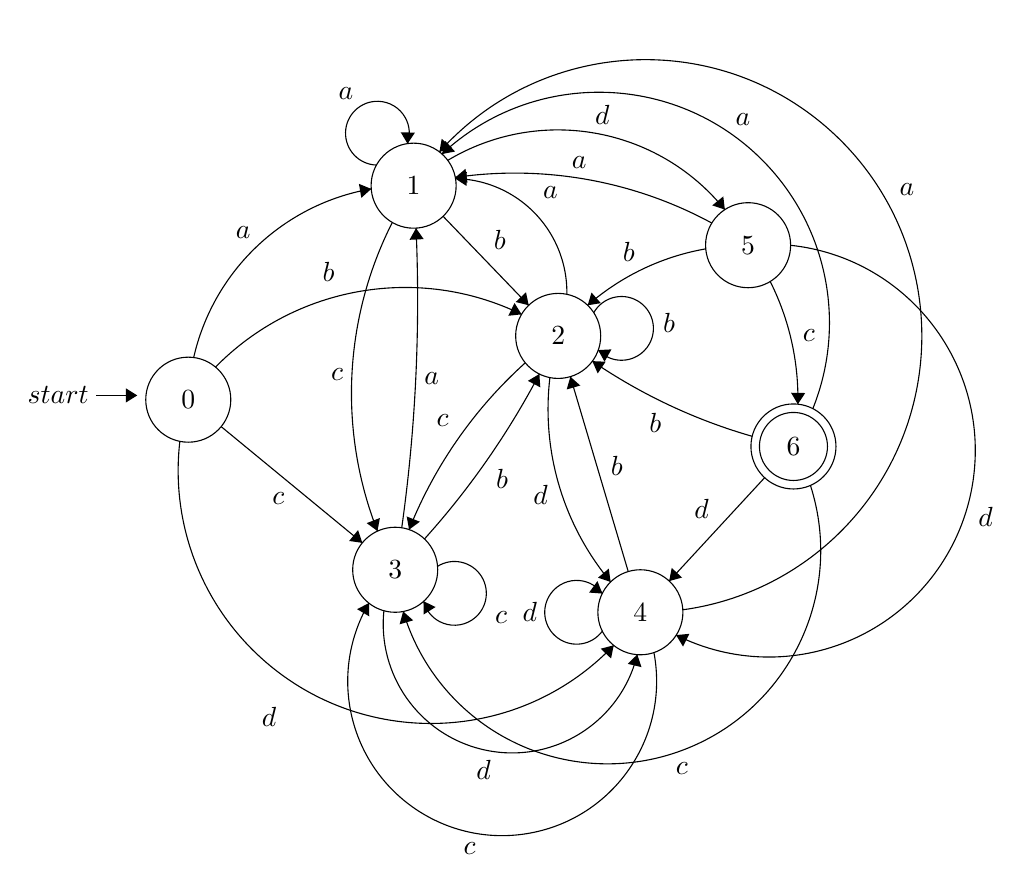
\begin{tikzpicture}[scale=0.18]
			\tikzstyle{every node}+=[fill=white,inner sep=0pt]
			\draw [black] (-2.6,-23.8) -- (0.3,-23.8);
			\draw (-3.1,-23.8) node [left] {$start$};
			\fill [black] (0.3,-23.8) -- (-0.5,-23.3) -- (-0.5,-24.3);
			\draw [black] (3.9,-24.1) circle (3);
			\draw (3.9,-24.1) node {$0$};
			\draw [black] (19.8,-9) circle (3);
			\draw (19.8,-9) node {$1$};
			\draw [black] (30,-19.6) circle (3);
			\draw (30,-19.6) node {$2$};
			\draw [black] (18.5,-36.1) circle (3);
			\draw (18.5,-36.1) node {$3$};
			\draw [black] (35.8,-39.1) circle (3);
			\draw (35.8,-39.1) node {$4$};
			\draw [black] (43.4,-13.2) circle (3);
			\draw (43.4,-13.2) node {$5$};
			\draw [black] (46.6,-27.4) circle (3);
			\draw (46.6,-27.4) node {$6$};
			\draw [black] (46.6,-27.4) circle (2.4);
			\draw [black] (33.919,-41.432) arc (-43.70358:-186.66407:17.839);
			\fill [black] (33.92,-41.43) -- (33,-41.67) -- (33.73,-42.36);
			\draw (11.22,-45.77) node [below] {$d\mbox{ }\mbox{ }\mbox{ }\mbox{ }\mbox{ }$};
			\draw [black] (6.22,-26) -- (16.18,-34.2);
			\fill [black] (16.18,-34.2) -- (15.88,-33.3) -- (15.25,-34.07);
			\draw (10.25,-30.59) node [below] {$c$};
			\draw [black] (5.821,-21.8) arc (135.53989:64.02493:18.753);
			\fill [black] (27.42,-18.08) -- (26.92,-17.28) -- (26.48,-18.18);
			\draw (15.1,-15.77) node [above] {$b\mbox{ }\mbox{ }\mbox{ }\mbox{ }$};
			\draw [black] (4.28,-21.129) arc (167.20329:99.84016:15.584);
			\fill [black] (16.81,-9.23) -- (15.94,-8.87) -- (16.11,-9.86);
			\draw (7.78,-12.8) node [above] {$a$};
			\draw [black] (17.19,-7.545) arc (268.59189:-19.40811:2.25);
			\draw (15.02,-2.94) node [above] {$a$};
			\fill [black] (19.37,-6.04) -- (19.89,-5.26) -- (18.89,-5.23);
			\draw [black] (32.505,-17.971) arc (150.77527:-137.22473:2.25);
			\draw (37.37,-18.68) node [right] {$b$};
			\fill [black] (32.82,-20.6) -- (33.27,-21.42) -- (33.76,-20.55);
			\draw [black] (21.479,-35.863) arc (122.28011:-165.71989:2.25);
			\draw (25.52,-39.48) node [right] {$c$};
			\fill [black] (20.5,-38.32) -- (20.5,-39.26) -- (21.35,-38.73);
			\draw [black] (17.251,-33.374) arc (-158.59999:-206.89281:26.653);
			\fill [black] (17.25,-33.37) -- (17.42,-32.45) -- (16.49,-32.81);
			\draw (14.87,-22.35) node [left] {$\mbox{ }\mbox{ }\mbox{ }\mbox{ }\mbox{ }\mbox{ }\mbox{ }\mbox{ }c$};
			\draw [black] (22.205,-7.215) arc (120.91152:38.90637:15.136);
			\fill [black] (41.76,-10.69) -- (41.65,-9.76) -- (40.87,-10.39);
			\draw (33.11,-4.71) node [above] {$d$};
			\draw [black] (22.741,-8.501) arc (88.91183:-1.11524:8.025);
			\fill [black] (22.74,-8.5) -- (23.53,-9.02) -- (23.55,-8.02);
			\draw (28.9,-9.49) node [right] {$a$};
			\draw [black] (19.478,-33.265) arc (158.24167:132.00767:31.599);
			\fill [black] (19.48,-33.27) -- (20.24,-32.71) -- (19.31,-32.34);
			\draw (22.31,-25.55) node [left] {$c$};
			\draw [black] (33.704,-36.958) arc (-140.13045:-186.74081:19.012);
			\fill [black] (33.7,-36.96) -- (33.57,-36.02) -- (32.81,-36.66);
			\draw (29.3,-30.79) node [left] {$\mbox{ }\mbox{ }d$};
			\draw [black] (35.581,-42.078) arc (-13.66199:-186.01371:9.092);
			\fill [black] (35.58,-42.08) -- (34.91,-42.74) -- (35.88,-42.97);
			\draw (24.73,-49.48) node [below] {$d$};
			\draw [black] (19.971,-11.995) arc (2.52337:-8.01617:115.218);
			\fill [black] (19.97,-12) -- (19.51,-12.82) -- (20.51,-12.77);
			\draw (20.52,-22.61) node [right] {$a$};
			\draw [black] (21.88,-11.16) -- (27.92,-17.44);
			\fill [black] (27.92,-17.44) -- (27.73,-16.52) -- (27,-17.21);
			\draw (25.43,-12.83) node [right] {$b$};
			\draw [black] (28.674,-22.291) arc (-27.74002:-42.01064:57.083);
			\fill [black] (28.67,-22.29) -- (27.86,-22.77) -- (28.74,-23.23);
			\draw (25.58,-29.72) node [right] {$b$};
			\draw [black] (22.741,-8.416) arc (98.28712:61.53076:29.155);
			\fill [black] (22.74,-8.42) -- (23.6,-8.8) -- (23.46,-7.81);
			\draw (33.11,-7.86) node [above] {$a\mbox{ }\mbox{ }\mbox{ }\mbox{ }\mbox{ }$};
			\draw [black] (32.077,-17.44) arc (131.12228:99.93712:17.189);
			\fill [black] (32.08,-17.44) -- (33.01,-17.29) -- (32.35,-16.54);
			\draw (34.99,-14.37) node [above] {$b$};
			\draw [black] (44.959,-15.759) arc (26.66951:-1.27035:18.386);
			\fill [black] (46.91,-24.42) -- (47.43,-23.63) -- (46.43,-23.61);
			\draw (47.22,-19.58) node [right] {$c$};
			\draw [black] (46.395,-13.207) arc (83.9582:-116.6654:14.567);
			\fill [black] (38.32,-40.71) -- (38.81,-41.52) -- (39.26,-40.62);
			\draw (59.61,-32.38) node [right] {$d$};
			\draw [black] (44.57,-29.6) -- (37.83,-36.9);
			\fill [black] (37.83,-36.9) -- (38.74,-36.65) -- (38.01,-35.97);
			\draw (40.67,-31.79) node [left] {$d$};
			\draw [black] (43.687,-26.684) arc (-106.00985:-124.32589:39.144);
			\fill [black] (32.41,-21.38) -- (32.79,-22.25) -- (33.35,-21.42);
			\draw (36.85,-24.99) node [below] {$b$};
			\draw [black] (47.797,-30.145) arc (17.84688:-163.44093:15.041);
			\fill [black] (19.06,-39.04) -- (18.81,-39.95) -- (19.77,-39.67);
			\draw (38.73,-49.67) node [below] {$c$};
			\draw [black] (21.796,-6.766) arc (132.94565:-21.89007:16.264);
			\fill [black] (21.8,-6.77) -- (22.72,-6.59) -- (22.04,-5.85);
			\draw (43.03,-4.76) node [above] {$a$};
			\draw [black] (33.12,-40.423) arc (324:36:2.25);
			\draw (28.55,-39.1) node [left] {$d$};
			\fill [black] (33.12,-37.78) -- (32.77,-36.9) -- (32.18,-37.71);
			\draw [black] (36.754,-41.934) arc (10.72301:-210.39871:10.898);
			\fill [black] (16.65,-38.45) -- (15.81,-38.88) -- (16.67,-39.39);
			\draw (23.75,-55.29) node [below] {$c$};
			\draw [black] (34.94,-36.22) -- (30.86,-22.48);
			\fill [black] (30.86,-22.48) -- (30.6,-23.38) -- (31.56,-23.1);
			\draw (33.67,-28.75) node [right] {$b$};
			\draw [black] (21.619,-6.618) arc (138.23159:-82.24481:19.498);
			\fill [black] (21.62,-6.62) -- (22.52,-6.35) -- (21.78,-5.69);
			\draw (54.06,-9.29) node [right] {$a$};
			\end{tikzpicture}
		
	
		\caption{\dfasr for  $\mathcal{P}=a ; d ; c$ with $\Sigma=\{a,b,c,d\}$, and order $m=1$.}
	\label{fig:dfa_adc}
	\end{centering}
\end{figure}






%(note that the DFA has no dead states since we need to handle streams and not strings).

\item  Given a constructed \textit{m-unambiguous} DFA for the pattern $\mathcal{P}$, and  assuming that the input events stream $s=\langle e_1,e_3,...,e_t,...\rangle$ is a $m$-order homogeneous Markov sequence, where $m \geq 1$.  ~\citet{nuel_pattern_2008} showed that the sequence of states of the DFA that generated by consuming the input events stream $s$ is a first-order homogeneous Markov chain, which is represented by $\langle q_{0},q_{1},...,q_{t},...\rangle$, where $q_{0}=s$ and $q_{t}=\delta(q_{t-1},e_{t})$. We denote by \pmcmr the derived Markov chain associated with a pattern $\mathcal{P}$ that is called a Pattern Markov Chain (PMC) of order $m$ \cite{nuel_pattern_2008}. In other words, we perform a direct mapping of the states of the DFA to states of a homogeneous Markov chain and the transitions of the DFA to transitions of the Markov chain. Thus, the terms \textit{m-unambiguous} DFA of a pattern and the corresponding \pmcmr  will be used interchangeably. 

\par Furthermore, the \pmcmr model is characterized by a $\vert Q \vert \times \vert Q \vert$ transition probability matrix $\Pi$ where $Q$ is the set of states of the  \textit{m-unambiguous} DFA. Figure ~\ref{fig:pmc} depicts the PMC of order 1 for the generated DFA of Figure ~\ref{fig:dfa_adc}.

%\par The next step is to derive a Markov chain that will be able to provide a probabilistic description of the DFA's run-time behavior.
%\par Towards this goal, we use Pattern Markov Chains, as was proposed in \cite{nuel_pattern_2008}.
%, it can be shown that there is a direct mapping of the states of the DFA to states of a Markov chain and the transitions of the DFA to transitions of the Markov chain.
%\par The transition probabilities of the Markov chain are the occurrence probabilities of the various event types.
%On the other hand, if the occurrence probabilities of the events are dependent on some of the previous events  seen in the stream (i.e., the stream is generated by an $m^{th}$ order Markov process), we might need to perform a more complex transformation 
%(see \cite{nuel_pattern_2008} for details)
%in order to obtain a ``proper'' Markov chain.
%The transition probabilities are then conditional probabilities on the event types.
%In any case,
%we call such a derived Markov chain a Pattern Markov Chain (PMC) of order $m$
%and denote by \pmcmr , where $\mathcal{P}$ is the initial pattern and $m$ the assumed order.
 
\end{itemize}


%\begin{figure}[!ht]
%\begin{centering}
%
%\includegraphics[width=0.35\textwidth]{./chapters/figures/forecasting/dfasr.pdf}
%\label{fig:dfa_adc}
%
%\hfill
%
%\includegraphics[width=0.35\textwidth]{./chapters/figures/forecasting/pmcr1.pdf}
%\label{fig:mc_adc}
%
%%\hfill
%\caption{DFA and PMC for $\mathcal{P}=a ; c ; c$,  $\Sigma=\{a,b,c\}$, and order $m=1$.}
%\label{fig:dfa_mc}
%\end{centering}
%\end{figure}

\begin{figure}[!h]
	\begin{centering}
		
	
			
			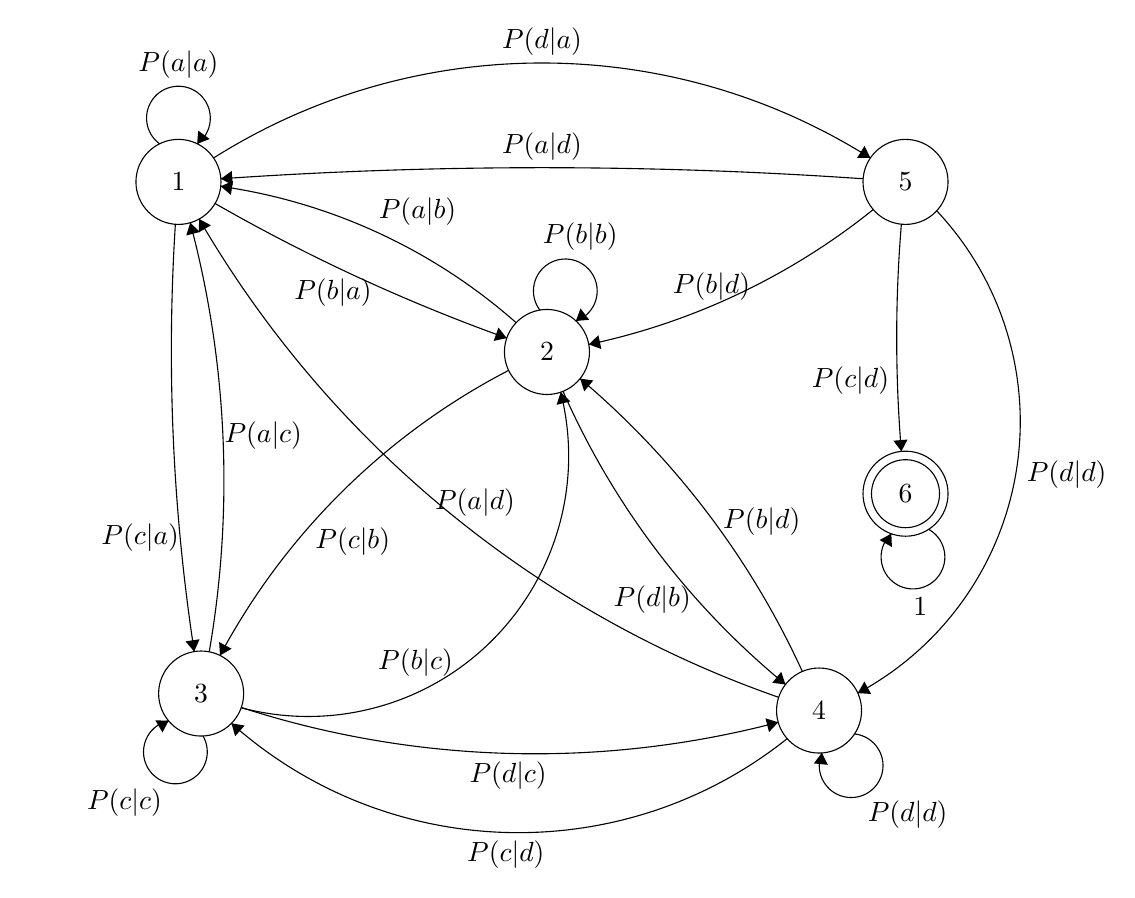
\begin{tikzpicture}[scale=.18]
			\tikzstyle{every node}+=[inner sep=0pt]
			\draw [black] (4.6,-12.2) circle (3);
			\draw (4.6,-12.2) node {$1$};
			\draw [black] (30.6,-24.2) circle (3);
			\draw (30.6,-24.2) node {$2$};
			\draw [black] (6.2,-48.3) circle (3);
			\draw (6.2,-48.3) node {$3$};
			\draw [black] (49.8,-49.5) circle (3);
			\draw (49.8,-49.5) node {$4$};
			\draw [black] (55.9,-12.2) circle (3);
			\draw (55.9,-12.2) node {$5$};
			\draw [black] (55.9,-34.2) circle (3);
			\draw (55.9,-34.2) node {$6$};
			\draw [black] (55.9,-34.2) circle (2.4);
			\draw [black] (3.277,-9.52) arc (234:-54:2.25);
			\draw (4.6,-4.95) node [above] {$P(a|a)$};
			\fill [black] (5.92,-9.52) -- (6.8,-9.17) -- (5.99,-8.58);
			\draw [black] (30.106,-21.253) arc (217.25487:-70.74513:2.25);
			\draw (32.95,-17.1) node [above] {$P(b|b)$};
			\fill [black] (32.64,-22.01) -- (33.58,-21.93) -- (32.97,-21.13);
			\draw [black] (6.328,-51.286) arc (30.18097:-257.81903:2.25);
			\draw (0.79,-55) node [below] {$P(c|c)$};
			\fill [black] (3.91,-50.22) -- (2.97,-50.19) -- (3.47,-51.05);
			\draw [black] (5.714,-45.34) arc (-171.29151:-183.63296:140.372);
			\fill [black] (5.71,-45.34) -- (6.09,-44.47) -- (5.1,-44.62);
			\draw (4.67,-37.32) node [left] {$\mbox{ }\mbox{ }\mbox{ }\mbox{ }\mbox{ }\mbox{ }\mbox{ }\mbox{ }P(c|a)$};
			\draw [black] (7.079,-10.512) arc (122.2697:57.7303:43.399);
			\fill [black] (53.42,-10.51) -- (53.01,-9.66) -- (52.48,-10.51);
			\draw (30.25,-3.31) node [above] {$P(d|a)$};
			\draw [black] (7.583,-12.513) arc (81.8726:48.57712:40.066);
			\fill [black] (7.58,-12.51) -- (8.3,-13.12) -- (8.45,-12.13);
			\draw (21.47,-15.28) node [above] {$P(a|b)$};
			\draw [black] (7.532,-45.612) arc (151.86818:117.42301:48.336);
			\fill [black] (7.53,-45.61) -- (8.35,-45.14) -- (7.47,-44.67);
			\draw (16.9,-36.53) node [below] {$P(c|b)$};
			\draw [black] (47.431,-47.66) arc (-129.36992:-156.24084:55.875);
			\fill [black] (47.43,-47.66) -- (47.13,-46.77) -- (46.5,-47.54);
			\draw (40.79,-41.65) node [left] {$P(d|b)$};
			\draw [black] (46.917,-50.329) arc (-75.2387:-107.9144:67.363);
			\fill [black] (46.92,-50.33) -- (46.02,-50.05) -- (46.27,-51.02);
			\draw (27.86,-53.1) node [below] {$P(d|c)$};
			\draw [black] (5.432,-15.082) arc (14.88666:-9.81113:70.847);
			\fill [black] (5.43,-15.08) -- (5.15,-15.98) -- (6.12,-15.73);
			\draw (7.81,-30.13) node [right] {$P(a|c)$};
			\draw [black] (27.764,-23.221) arc (-109.71785:-119.83243:128.561);
			\fill [black] (27.76,-23.22) -- (27.18,-22.48) -- (26.84,-23.42);
			\draw (15.5,-19.0) node [below] {$P(b|a)$};
			\draw [black] (31.568,-27.036) arc (14.17669:-104.88549:18.382);
			\fill [black] (31.57,-27.04) -- (31.28,-27.93) -- (32.25,-27.69);
			\draw (24,-46.09) node [left] {$P(b|c)$};
			\draw [black] (7.592,-11.979) arc (93.95767:86.04233:328.286);
			\fill [black] (7.59,-11.98) -- (8.42,-12.42) -- (8.36,-11.43);
			\draw (30.25,-10.7) node [above] {$P(a|d)$};
			\draw [black] (53.622,-14.151) arc (-51.2137:-78.03555:47.886);
			\fill [black] (33.55,-23.67) -- (34.44,-23.99) -- (34.23,-23.02);
			\draw (44.97,-20.61) node [above left] {$P(b|d)$};
			\draw [black] (55.607,-31.214) arc (-175.27936:-184.72064:97.384);
			\fill [black] (55.61,-31.21) -- (56.04,-30.38) -- (55.04,-30.46);
			\draw (54.78,-27.2) node [above left] {$P(c|d)$};
			\draw [black] (58.099,-14.237) arc (43.2333:-61.80904:21.727);
			\fill [black] (52.53,-48.27) -- (53.47,-48.33) -- (53,-47.45);
			\draw (64.42,-32.85) node [right] {$P(d|d)$};
			\draw [black] (52.291,-51.151) arc (84.18903:-203.81097:2.25);
			\draw (56.05,-55.84) node [below] {$P(d|d)$};
			\fill [black] (50,-52.48) -- (49.43,-53.23) -- (50.42,-53.33);
			\draw [black] (47.55,-51.483) arc (-51.43786:-131.71524:30.426);
			\fill [black] (8.34,-50.4) -- (8.6,-51.31) -- (9.27,-50.56);
			\draw (27.7,-58.68) node [below] {$P(c|d)$};
			\draw [black] (32.939,-26.078) arc (49.80232:24.58692:59.422);
			\fill [black] (32.94,-26.08) -- (33.23,-26.98) -- (33.87,-26.21);
			\draw (43,-36.14) node [right] {$P(b|d)$};
			\draw [black] (46.949,-48.567) arc (-109.23723:-149.82312:76.434);
			\fill [black] (6.06,-14.82) -- (6.03,-15.77) -- (6.89,-15.26);
			\draw (22.67,-34.85) node [right] {$P(a|d)$};
			\draw [black] (57.526,-36.707) arc (60.70628:-227.29372:2.25);
			\draw (56.94,-41.49) node [below] {$1$};
			\fill [black] (54.9,-37.02) -- (54.07,-37.47) -- (54.94,-37.96);
			\end{tikzpicture}
			
		
		
		%\hfill
		\caption{\pmconer for $\mathcal{P}=a ; d ; c$ with $\Sigma=\{a,b,c,d\}$, and order $m=1$.}
		\label{fig:pmc}
	\end{centering}
\end{figure}





%\end{comment}

\subsubsection*{Constructing the Pattern Prediction Model}
\label{sec:pmc_prediction}

~\citet{alevizos2017event} proposed to use the constructed \pmcmr to build a probabilistic prediction model that describes the DFA's run-time behavior. The method is based on calculating the \textit{waiting-time} distributions. Given a specific state of the \pmcmr, a \textit{waiting-time} distribution provides the probability of reaching an absorbing state in $n$ transitions from the current state. So by mapping the final states of the DFA to absorbing states of the \pmcmr by adding self-loops with probabilities equal to $1.0$. Therefore, we can calculate the probability of reaching a final state in $n$ transitions, which means predicting a full match of the defined pattern $\mathcal{P}$.

\par We denote by $W_{\mathcal{P}}(q)$ the waiting-time random variable that represents the number of transitions from a current state $q$ of DFA to reach a final state \cite{alevizos2017event}, where it also represents the expected number of future events from the current time event to a full match of the pattern $\mathcal{P}$, which is given by 

\begin{equation*}
W_{\mathcal{P}}(q)=inf\{n: q_{0},q_{1},...,q_{n}, q_{0}=q, q \in Q \backslash F, q_{n} \in F\}
\end{equation*}

where $Q$ is the set of states of the DFA, and $F$ the set of the  all final states. However, the \textit{waiting-time} distribution of the $W_{\mathcal{P}}(q)$ random variable can be computed based on the transition probability matrix $\Pi$ of the \pmcmr, where it has $h$ non-final states and $d$ final states (absorbing states) \cite{alevizos2017event}, then the distribution is calculated by the following equation 

\begin{equation*}
P(W_{\mathcal{P}}(q)=n)=\boldsymbol{\xi_{q}}\boldsymbol{N}^{n-1}(\boldsymbol{I}-\boldsymbol{N})\boldsymbol{1}
\end{equation*}
where $\boldsymbol{N}$ is $h \times h$ matrix that obtained by re-arranging the transition matrix $\Pi$ to include transitions between the non-final states of the DFA, $\boldsymbol{I}$ is an identity matrix of size $h \times h$, and  $\boldsymbol{1}$ is a $h$-dimensional vector of ones. The $\boldsymbol{\xi_{q}}$ is $1 \times h$ row of elements that contains zeros except $1.0$ in the cell corresponding to $q$. 
\par Finally, the model provides the prediction reports in the form of intervals i.e.,  $I=(\mathit{start},\mathit{end})$. Which means that the DFA is expected to reach a final state  after future transitions (number of events $n$) between $\mathit{start}$ and $\mathit{end}$ with probability $P(I)$ at least some constant threshold $\theta_{p}$ that defined by the user, given by:
\begin{equation*}
P(I)=\sum_{n \in I}{P(W_{\mathcal{P}}(q)=n)}\ where\  P(I) \geq \theta_{p} 
\end{equation*}
where $P(I)$ equals the sum of probabilities of all number of future events $n$ that fall within $I$ ($start\leq n\leq end$). Furthermore, the length of the intervals ($spread(I) = end - start$)  can be restricted to not be greater than a maximum spread threshold $\theta_{s}$ ($spread(I)\leq \theta_{s}$)



\begin{figure}[H]
	\begin{centering}
		\center
		\includegraphics[width=\textwidth,keepaspectratio]{chapters/figures/new_wt.png}
		
		
		\caption{Waiting-time distribution for
			$\mathcal{P}=a ; d ; c$, $\Sigma=\{a,b,c,d\}$, $m=1$, $\theta_{p}=0.5\ and\ \theta_{s}=20$.}
		\label{fig:wt1}
	\end{centering}
\end{figure}

\par These intervals are estimated by a single-pass algorithm that scans a waiting-time distribution and finds the smallest (in terms of length) interval that exceeds the $\theta_{p}$ and has a spread  not greater that $\theta_{s}$. For example, Figure~\ref{fig:wt1} shows the \textit{waiting-time} distributions for all non-final states of the DFA presented in Figure~\ref{fig:wt1}, and the generated intervals are depicted in Figure~\ref{fig:predictionsIntervals}.


\begin{figure}[H]
	\begin{centering}
		\center
			\includegraphics[width=\textwidth,keepaspectratio]{chapters/figures/new_prediction_intervals.png}
					
		\caption{Example of the computed prediction intervals for
			$\mathcal{P}=a ; d ; c$, $\Sigma=\{a,b,c,d\}$, $m=1$, $\theta_{p}=0.5\ and\ \theta_{s}=20$.}
		\label{fig:predictionsIntervals}
	\end{centering}
\end{figure}

\par The proposed method assumes that the transition probability matrix $\Pi$ is available to build the prediction intervals. However, this is not true in the real-world applications.
Therefore, it is essential to learn the values of the \pmcmr's transition probability matrix in order apply this method. One common way, is to use the maximum-likelihood estimator to learn the transition probabilities as illustrated in Section ~\ref{sec:theoretical}. 

\par This model is performing the learning over an event stream $s$, which is usually has a slow convergence to a sufficiently good model. Where in the case of multiple event streams, a unique model associated with each stream is needed. Accordingly, we present in this work, a technique to share information among the \pmcmr predictors over multiple input event streams (i.e., distributed learning of the transition probability matrix).

\section{Pattern Prediction over Multiple Event Streams}

We extend the pattern prediction problem over a single event stream to the case of multiple distributed input event streams, where there is an associated prediction model for each event stream. We further present our proposed cooperative learning based approach by using a distributed online prediction protocol \cite{kamp2014communication} to synchronize the distributed prediction models in a communication-efficient manner. 


\subsection{Extended Problem Formulation}

\par In this section, we extend the problem of pattern prediction over a single event stream to consider the setting where there are multiple input event streams. Let $O = \{ o_1, ..., o_k\}$ be a set of \emph{$K$} objects/entities (e.g., moving objects), each of which is generating an event stream $s_i$, hence, we have a set of real-time input event streams $S = \{ s_1, ..., s_k\}$, where these streams are produced independently from the same distribution.


 \par $\mathcal{P}$ is a user-defined pattern given in the form of regular expression, which is monitored in every stream $s_i \in S$. Then, we have a system consists of \emph{$K$} local predictor (learner) nodes $n_1,n_2\dots,n_k$, each of which receives an input event stream $s_i\in S$ that is associated with a single object $o_i \in O$.

\par  The goal is to provide online predictions about the completion of the pattern $\mathcal{P}$ within each stream $s_i$. Each node maintains a local prediction model $f_i$. Then for each new arriving event tuple  $e_t \in s_i$, the $f_i$ model provides an online prediction interval about the future full match of the pattern $\mathcal{P}$.

\par In other words, we have separated running instances of an online prediction algorithm on distributed nodes for \emph{$K$} input event streams. For example, massive streams of events that describe trajectories of group of moving vessels in the context of maritime monitoring, where there is one predictor node for each vessel's event stream.
  
  
  \par In this work, we employ the \pmcmr models on the distributed predictor nodes, each model is associated with a particular event stream. While these predictors can work in isolation with no communication with other local predictors, such non-cooperative way leads to inefficiency in terms of learning convergence and predictive performance among all predictors. Thus, in this work, we propose to use the distributed online prediction protocol \cite{kamp2014communication} to enable the communication among the local predictors to synchronize their models.     
%
%The defined pattern $\mathcal{P}$ is monitored over each event stream $s_i$  by a  predictor nodes  $n_i$  that maintains a local prediction model $f_i$, where there is one node for each vessel's event stream.  The prediction model $f_i$ gives the ability to provide an online predictions about when the pattern will be completed in the form of an expected number of future events before a full match does occur.

\subsection{The Proposed Method}
\label{sec:proposed_approach}

\par This work proposes a scalable and distributed prediction system for user-defined patterns over multiple massive input event streams. The system  uses the PMC forecasting method \cite{alevizos2017event} as the base prediction model, where there is a \pmcmr model associated with each input event stream $s_i$ on a predictor node $n_i$. And it employs the distributed online learning protocol \cite{kamp2014communication} to exchange information among the distributed predictors of the input event streams, which allows to synchronize the parameters of their prediction models, which are represented by the transition matrices.

%
%Thus, the prediction model $f_i$ on a predictor node is represented by \pmcmr and its associated DFA.

\subsection*{Distributed Online Learning for Pattern Prediction}

\par In what follows, we describe the details of adapting the distributed online learning protocol \cite{kamp2014communication} with the pattern prediction (\pmcmr) models. This protocol provides a communication-efficient dynamic synchronization scheme based on a periodic static scheme.


\par Algorithm~\ref{algonline:dol} presents the distributed online prediction protocol by dynamic model synchronization on both the predictor nodes and the coordinator. We refer to the PMC's transition matrix $\boldsymbol{\Pi}_i$ on predictor node $n_i$ by $w_i$, which represents the parameters of the local prediction model $f_i$. 

\par That is, when a predictor $n_i:\ i \in[k]$ observes an event $e_j$ it revises its internal model state ($w_i$) and provides a prediction report. Then it checks the local conditions, by checking the local model divergence from a reference model $w_r$ after consuming a predefined number of events (batch size $b$), to decide whether there is a need to synchronize its local model with the coordinator [or not]. $w_r$ is maintained in the predictor node as a copy of the last computed aggregated model $\hat{w}$ from the previous full synchronization step, which is shared among all distributed predictors.
%define delta%
 \par Let $\Delta$ be a predefined divergence threshold parameter. Then, by monitoring the local condition $(\|w_i - w_r\|^2 > \Delta)$ on all local predictors, we have a guarantee that if none of the local conditions is violated, the divergence (i.e., variance of local models $\delta(w)=\frac{1}{k} \sum_{j=1}^{k}\|w_i - \hat{w}\|^2$) does not exceed the threshold $\Delta$ \cite{kamp2014communication}. This is the key point of this protocol that reduces the communication overhead in comparison to the static based communication scheme, where the predictors always communicate periodically after observing a fixed number ($b$) of events ~\cite{dekel2012optimal}.  

\par On the other hand, the coordinator receives the parameters of prediction models from the predictor nodes that requested for model synchronization (violation). Then it tries to keep incrementally querying other nodes for their local prediction models until reaching out all nodes have been queried, or the variance of the aggregated parameters $\hat{w}$ that is computed from the already received models is less or equal than the divergence threshold $\Delta$. The coordinator uses a synchronization operation to compute the parameters of a global model  $\hat{w}$. Finally, $\hat{w}$ is sent back to the predictor nodes that sent their models after the violation or have been queried by the coordinator. 

\begin{algorithm}[h]
	\caption{Communication-efficient Distributed Online Learning \cite{kamp2014communication}.} 
	\begin{algorithmic}[1] 
		
		\Statex \Indm  \textbf{Predictors:}
		\Statex \Indp node $n_i$: at observing event $e_j$
		
		\Statex \Indp update the parameters of the local prediction model $w_i$ and provide a prediction interval $I$ \;
	 

		\Statex \If {$j\mod b = 0\ and\ \|w_i - w_r\|^2 > \Delta$}  
		\Statex send  $w_i$ to the Coordinator (violation) \;
		\Statex \Indm \textbf{Coordinator}:
		\Statex \Indp receive parameters of local models with violation 
		 $B=\{w_i\}_{i=1}^m$ \;
	
	
		\Statex \While{$|B| \neq k $ and $\frac{1}{|B|} \ \sum_{w_i\in  \Pi}\|w_i - \hat{w}\|^2 > \Delta$}{
			
			 \Statex  \hspace{\algorithmicindent} add other nodes that have not reported violation for \Statex \hspace{\algorithmicindent} their models $ B \gets \{w_l : w_l \notin B\ and\ l \in [k]\}$    \;
			\Statex  \hspace{\algorithmicindent} receive models from nodes in $B$\;
	}
        \Statex
		\Statex compute a new global model $\hat{w}$ \;
		\Statex send $\hat{w}$ to all the predictors in $B$ and set $w_{1}\dots w_{m}=\hat{w} $\; 
		\Statex \If {$|B| = k$}{
		\Statex  \hspace{\algorithmicindent} set a new reference model $w_r	\gets \hat{w}$ \; }
	
	\end{algorithmic}
	\label{algonline:dol}
\end{algorithm}


\par  We use this protocol for the pattern prediction models, which are internally based on the \pmcmr. This allows the distributed \pmcmr predictors for multiple event streams to synchronize their models (i.e., the transition probability matrix of each predictor), and learn a shared model in a communication-efficient way. 


\subsection*{Learning a Global Transition Probability Matrix}

\par We propose a \textit{synchronization operation} for the transition probability matrices ($w_i=\boldsymbol{\Pi}_i :i \in[k]$) of the $k$ distributed \pmcmr predictors. The operation is based on distributing the maximum-likelihood estimation \cite{anderson1957statistical} for the transition probabilities of the \pmcmr models. 
Let $\pi_{i,j}$ the transition probability from state $i$ to state $j$ 
and $n_{k,i,j}$ the number of transitions from state $i$ to state $j$ on node $k$. Then, the global estimation $\hat{\pi}_{i,j}$ for $p_{i,j}$ is described by:

\begin{equation}
\label{eq:dis_pi_estim}
\hat{\pi}_{i,j} = \frac{\sum_{k \in K} n_{k,i,j}}{\sum_{k \in K} \sum_{l \in L} n_{k,i,l}}
\end{equation}

That is,  $\hat{\Pi}$ is the global transition probability matrix that will be shared among all \pmcmr predictors. 
\par Moreover, we measure the divergence of the local models from the reference model $\|w_i - w_r\|^2$ by calculating the sum of square difference between the local transition probability matrix $\Pi_i$ and the reference transition matrix $\Pi_r$:
\begin{equation*}
\label{eq:dis_pi_varinace}
\|w_i - w_r\|^2=|\Pi_i - \Pi_r\|^2=\sum_{l,j} (\pi{i,l,j} -\pi{r,l,j})^2
\end{equation*}

Where $\pi{i,l,j}$ is the transition probability from state $l$ to state $j$ in the $\Pi_i$, and the $\pi{r,l,j}$ the reference transition probability.



\subsection{Theoretical Analysis}
\label{sec:theoretical}
 %probability gaurantee %
 %SAY something about the relation between transition probabilities and prediction%
 In this section, we present preliminaries of Markov chain and the maximum like-hood estimator of the transition probabilities, and we describe the theoretical properties of our proposed synchronization operator and its relation with the maximum likelihood estimator. 
 
 % take the mc matrix from pmc paper and try to derive the varince 
 
 \subsubsection*{Preliminaries}
 In this section, we first present some definitions related to Markov chain theory, 
where the theoretical definitions presented  are based 
on the work described in \cite{bertsekas2002introduction,Billingsley1961,anderson1957statistical,howard2012dynamic}.

\begin{definition}
	Let $\{s_0, s_1, \ldots s_n\}$ be a sequence of random variables as \textbf{Markov chain}, where $s_i$ belongs to a finite state space $\mathbf{S =\{1,\ldots m\}}$ and represents the observed state of the chain at time $i$. Let the transition probabilities of the Markov chain $p_{ij}(t+1)$ such that $i,j \in S$ and $t=0,\ldots, n$, where  $p_{ij}(t+1)$ is the probability of the state $j$ at time $t+1$, given state $i$ at time $t$, where the sequence $\{s_0, s_1, \ldots s_n\}$ satisfies the \textbf{Markov property} 
	
	\begin{equation}
	\begin{aligned}
	P(s_{t+1}=j|s_{t}=i,s_{t-1}=i_{t-1},\ldots ,s_{0}=i_{0})=P(s_{t+1}=j|s_{t}=i)\\
	\forall i,j,i_{t-1},i_{0} \in S
	\end{aligned}
	\end{equation}

	
	Thus, the probability of moving to a future state only depends on the current  state (first-order Markov chain). While for higher order $m$ Markov chains the conditional probabilities can be modeled to be dependent on the last $m$ states. 
	
	When the conditional probabilities $P(s_{t+1}=j|s_{t}=i)$ are independent of the time $t$, the Markov chain is called \textbf{homogeneous} such that $p_{ij}:=P(s_{t+1}=j|s_{t}=i)$.
	

	
\end{definition}

The transition probabilities of the Markov chain are represented by a $m \times m$ matrix that called \textbf{transition probability matrix} $\boldsymbol{\Pi}$ with $p_{ij}$ elements


\begin{equation}
\label{eq:matrix_example}
\boldsymbol{\Pi} = 
\begin{pmatrix} 
p_{1,1}	   &p_{1,2}  &. 		&. 		& . &  	p_{1,m} \\
p_{2,1}		   &.  & .		& .	    & .	& . \\
. 		   &.  & .		& .	    & .	& . \\
.		   &.  & .		& .		& .	& . \\
.		   &.  & .		& .		& .	& .\\
p_{m,1}	   & p_{m,1}	&.		& .	& .	&p_{m,m}
\end{pmatrix}
\end{equation}

where $0 \leq p_{i,j}\leq 1 $ and the rows sum up to one 
\begin{equation}
\sum_{j=1}^{m} p_{i,j}= 1\ \ \ \ \ \ \ \ \ i=1,2 \ldots m
\end{equation}

\textbf{Learning the Transition Probability Matrix}. As mentioned in Section ~\ref{sec:pmc_prediction}, we rely on the transition probability matrix of \pmcmr to build the predictions table. However, in practice the underlying  transition probability matrix is unknown, and desirable to estimate or learn it form the observed sequence $\{s_0, s_1, \ldots s_n\}$. The maximum likelihood estimator (MLE) is a common method to estimate the transition probability matrix \cite{anderson1957statistical}.


\begin{definition}
	Let $\boldsymbol{\Pi}$ is the transition probability matrix of a single Markov chain with a set of states $S$, 
	$\pi_{i,j}$ the transition probability from state $i$ to state $j$,
	$n_{i,j}$ the number of observed transitions from state $i$ to state $j$,
	then the maximum likelihood estimator finds $\boldsymbol{\hat{\Pi}}$ as an estimate for $\boldsymbol{\Pi}$, where its elements $\hat{p}_{i,j}$ are
	\begin{equation}
	\label{eq:pi_estim}
	\hat{p}_{i,j}=\frac{n_{i,j}}{\sum_{l \in S} n_{i,l}}=\frac{n_{i,j}}{n_{i}}
	\end{equation}
	
\end{definition} 


	The maximum likelihood estimates of transition probabilities of a single sequence $\{s_0, s_1, \ldots s_n\}$   are obtained based on the observed transitions between the states of the chain. That is, the maximum likelihood estimates are basically the count of transitions from $i$ to $j$ divided by the total count of the chain being in state $i$.  
	
	\par ~\citet{anderson1957statistical} have shown that 
	
	
%	\begin{equation}
%	\label{eq:lim_dist}
%	\lim_{n\to\infty} \sqrt{n}\ (\hat{p}_{i,j} - {p}_{i,j}) \sim \mathcal{N}(\mu,\,\sigma^{2}_{mle})\,.
%	\end{equation}

	\begin{equation}
	\begin{aligned}
	\label{eq:lim_dist}
	 \sqrt{n}\ (\hat{p}_{i,j} - {p}_{i,j}) \xrightarrow{d} \mathcal{N}(\mu,\,\sigma^{2}_{mle_n})\\
	 as\ n \xrightarrow{} \infty
	 \end{aligned}
	\end{equation}
Thus, the random variable $\sqrt{n}\ (\hat{p}_{i,j} - {p}_{i,j})$ has asymptotically normal distribution with mean $\mu=0$. Therefore, the MLE is an asymptotically normal. While the variance  $\sigma^{2}_{mle_n}$ is given by   




\begin{equation}
\begin{aligned}
\sigma^{2}_{mle_n}=\mathrm{Var}(\sqrt{n}\ (\hat{p}_{i,j} - {p}_{i,j})) = \frac {{p}_{i,j}\ (1- {p}_{i,j})} {\phi_{i}} \\
\text{s.t.}\ \phi_{i} = \sum_{l=1}^{m} \sum_{t=1}^{n} \eta_{l} \ p_{l,j}^{t-1}
\end{aligned}
\end{equation}

Where $p_{l,j}^{t-1}$ is the probability of state $j$ at time  $t-1$ given that the state $l$ at time $0$  ~\cite{anderson1957statistical}. We are interested in the variances of $(\hat{p}_{i,j} - {p}_{i,j})$ that represents the error in estimating ${p}_{i,j}$ by MLE, which is given by:

	\begin{equation}
\begin{aligned}
	\mathrm{Var} (\hat{p}_{i,j} - {p}_{i,j}) = \frac {\sigma^{2}_{mle_n}}{n} 
\end{aligned}
\end{equation}

It is clearly seen that variances are dropping as the sample size $n$ grows large.  In next, we will show that our proposed approach of synchronizing the maximum likelihood estimators over $k$ chains is preserving  a similar asymptotic behavior. 


\subsubsection{Properties of the Synchronization Operator}
 %in Equation ~\ref{eq:dis_pi_estim}% 
\par The proposed synchronization operator is basically aggregating the maximum likelihood estimates over $k$ observed sequences (i.e., sequences of the DFA states based on the consumed event streams), the operator estimates the maximum likelihood of the probabilities for a set of $k$ sequences, which are arranged in serial order as one large chain with length $ N=kn$ where we assume that all $k$ sequences have $n$ observations. For the sake of simplicity, we assume that the synchronization phase happens on batch size equals $n$ (i.e., $b=n$) the, then it follows that 
\begin{equation}
\label{eq:dis_pi_estim2}
	\begin{aligned}
\hat{\pi}_{i,j}=\frac{\sum_{k \in K} n_{k,i,j}}{\sum_{k \in K} \sum_{l \in L} n_{k,i,l}} = \hat{p}_{i,j}(N)\\\\
 where\ N = kn.
 \end{aligned}
\end{equation}
%This is equivalent to

\par Thus, this operation it allows to observe more samples, which is naturally producing a better estimates of the transition probabilities. In addition, our proposed synchronization operation of the $k$ transition matrices has the same proprieties as the maximum likelihood estimator over a serial sequence of all $k$ sequences, but with skipping $k-1$ transitions between each two consecutive sequences, which is in practice a small number that can be neglected comparing to the total transitions count $kn$. As result, the probabilities estimates of our estimator (i.e.,global) based on the proposed operation within the distributed online learning protocol have the same properties as maximum likelihood estimates, in particular, the the random variable $\sqrt{N}\ (\hat{\pi}_{i,j} - {p}_{i,j})$ has asymptotically normal distribution with mean $\mu=0$ following Equation ~\ref{eq:lim_dist} we have 

\begin{equation}
\begin{aligned}
\label{eq:lim_dist2}
\sqrt{N}\ (\hat{\pi}_{i,j} - {p}_{i,j}) \xrightarrow{d} \mathcal{N}(0,\,\sigma^{2}_{mle_N})\\
as\ N \xrightarrow{} \infty\\
where\ N = nk .\\
\end{aligned}
\end{equation}

So, 
\begin{equation}
\begin{aligned}
\label{eq:var_sync}
 \mathrm{Var} (\hat{\pi}_{i,j} - {p}_{i,j}) = \frac {\sigma^{2}_{mle_N}}{N} =  \frac {\sigma^{2}_{mle_n}}{kn}
\end{aligned}
\end{equation}


That is, since $N > n$ combining $k$ sequences, the variances  of our method estimates $\mathrm{Var} (\hat{\pi}_{i,j} - {p}_{i,j})$  are smaller than the estimates of MLE over an isolated sequence $\mathrm{Var} (\hat{p}_{i,j} - {p}_{i,j})$. Thus, it follows from the  Chebyshev's inequality \cite{feller1968introduction} that we have for the random variable $\hat{p}_{i,j} - {p}_{i,j}$, for any constant $c > 0$  

\[ \Pr\left( |(\hat{p}_{i,j} - {p}_{i,j}) - \mu| \geq c \right) \leq
\frac{\mathrm{Var} (\hat{p}_{i,j} - {p}_{i,j})}{c^2} \]


 where the mean $\mu=0$ is zero and the $\mathrm{Var} (\hat{p}_{i,j} - {p}_{i,j})$ equals  $\frac {\sigma^{2}_{mle_n}}{n}$, and therefore 
 
 \[ \Pr\left( |\hat{p}_{i,j} - {p}_{i,j}| \geq c \right) \leq
 \frac{\sigma^{2}_{mle_n}}{c^2 n} \]
 
 
$\hat{p}_{i,j} - {p}_{i,j}$  represents the deviation/error between the estimates of MLE over a single (i.e., isolated) sequence and the true probabilities. On the other hand, we can obtain, in the same way, the probability bound of deviations for our synchronization operator estimates as follows:

\[ \Pr\left( |\hat{\pi}_{i,j} - {p}_{i,j}| \geq c \right) \leq
\frac{\sigma^{2}_{mle_n}}{c^2 nk} \]


Using Equation ~\ref{eq:var_sync} we obtained the value $\mathrm{Var} (\hat{\pi}_{i,j} - {p}_{i,j})$. Since $k \ge 1$ we have that the variance of $(\hat{\pi}_{i,j} - {p}_{i,j})$  is less than or equal to the variance of $\hat{p}_{i,j} - {p}_{i,j}$

\[ 
\frac{\sigma^{2}_{mle_n}}{c^2 nk} \leq
\frac{\sigma^{2}_{mle_n}}{c^2 n}
 \]

This is equivalent to,for any constant $c > 0$ and $k \ge 1$ we have

\[ \Pr\left( |\hat{\pi}_{i,j} - {p}_{i,j}| \geq c \right) \leq
 \Pr\left( |\hat{p}_{i,j} - {p}_{i,j}| \geq c \right)
 \]

To summarize, our approach is based aggregating the MLE estimates over $k$ sequences, which speeds up the convergence to reach the true transition probabilities as result of the  smaller variances.

%The weak law of large
%numbers states that, if $X_1, X_2, X_3, \ldots$ are independent and identically
%distributed random variables with mean $\mu$ and standard deviation $\sigma$,
%then for any constant $\epsilon > 0$ we have 
%%
%\[ \lim_{n \rightarrow \infty} \Pr \left( \left| \frac{X_1 + X_2 + \cdots +
%	X_n}{n} - \mu \right| > \epsilon \right) = 0. \]
%Use Chebychev's inequality to prove the weak law of large numbers.

 
\subsubsection{Computing the Transition Matrix of the Underlaying Markov Chain}

\par In order to empirically study the asymptotic behavior of our proposed synchronization operator, we need to compute the transition probability matrix of the underlying Markov chain that the events belong to, and we introduce to calculate it  based on the transition matrix ($\Pi$) of \pmcmr that describes the Markov chain of the pattern.

~\citet{nuel_pattern_2008} showed in \textbf{Theorem 3} the relation between the elements  of 
$\Pi$ and the conditional probabilities of the $m-$order Markov chain $X=\{X_1, X_2, \ldots X_n\}$ described by 

\[ \Pi(p, q) =
\begin{cases}
P(X_{m+1}=b|X_1\ldots X_m=\delta^{-m}(p))     & \quad \text{if } \delta(p,q)=b \\
0  & \quad \text{if } p \notin  \delta(p,X)
\end{cases}
\]
Using this theorem, we can compute the transition probabilities of the Markov chain $X$. For example, the transition probability matrix of the DFA of  the pattern $\mathcal{P}=a ; d ; c$ over  $\Sigma=\{a,b,c,d\}$ can be represented by: 

\begin{equation*}
\label{eq:matrix}
\boldsymbol{\Pi} = 
\begin{Bmatrix} 
0 \\ 1 \\ 2 \\ 3 
\end{Bmatrix}
\begin{pmatrix} 
P(b)+P(c) 	& P(a) 		& 0 		& 0 \\
P(b) 		& P(a)		& P(c)		& 0 \\
P(b)		& P(a)		& 0			& P(c) \\
0			& 0			& 0			& 1.0
\end{pmatrix}
\end{equation*} 

%ADD figure example for the figure in the PMC section%


\section{Summary}

\par In this chapter, we addressed the problem of pattern prediction over \emph{$K$} event streams by extending the case of predicting  event patterns over a single stream, where there are \emph{$K$} distributed predictors.  We also described the used prediction model on each predictor, which is based on the event forecasting with pattern Markov chains method \cite{alevizos2017event}. We presented our approach to adapt the distributed online learning protocol \cite{kamp2014communication} that allows the predictors to synchronize their models in a communication-efficient way. Additionally, we provided the theoretical analysis of our approach by deriving a
 probabilistic guarantee on the learning efficiency. 
 
 \par In next chapter, we will introduce the high-level architecture of our pattern prediction system, which is composed of distributed \pmcmr predictors \cite{alevizos2017event} that communicate their models to a coordinator node based a dynamic synchronization scheme \cite{kamp2014communication}. The coordinator computes a global model using the proposed synchronization operation (Equation~\ref{eq:dis_pi_estim}) and shares among the predictors. We will also present the implementation details of the system based on Apache Flink and Apache Kafka.    
 
 
	
	

\chapter{System Overview}
\label{chapter:overview}


\par In this chapter, we present the architecture of the proposed system for pattern prediction over multiple input event streams in a scalable distributed setting. To build a scalable and distributed system, we implement the system on top of Apache Flink engine for distributed and large-scale stream processing. We also use Apache Kafka for the distributed communication and to ingest and emit the input/output data streams. In what follows we describe the building blocks of the proposed system and the important aspects of the implementation.

%ADD more details and interfacse structure%
%CHECK Towards Flexible Event Processing in Distributed Data Streams%
%SEE delevriable%
\section{System Architecture}
\label{sec:architecture}
The input to our system is an aggregated stream of events coming from a large number of  objects, which is continuously collected and fed into the system. In practice, the aggregated input events stream is composed of multiple event streams (partitions) from a set of objects. Our system allows the users to register a pattern $\mathcal{P}$ to be monitored over each event stream. The output stream consists of original input events along with  the prediction intervals of the full matches of monitored pattern $\mathcal{P}$, which are displayed to the end users. Figure~\ref{fig:architecture} presents an overview of our system architecture and its main components.      


\begin{figure}[h]
	\centering
	\includegraphics[width=\linewidth]{chapters/figures/system_v2.png}
	
	\caption{System architecture overview.}
	\label{fig:architecture}
\end{figure}

The system is composed of three main processing elements:   
\begin{itemize}
	
	\item The pre-processing operators: Operators receive the input event stream and perform filtering and ordering operations, before partitioning the input event stream to multiple event streams based on the associated object. 
	\item The predictor nodes (learners): Each predictor is responsible for maintaining a prediction model for an input event stream. Each prediction node is configured to handle an event stream from the same  object, in order to provide online predictions for the user-defined pattern $\mathcal{P}$.  
	\item The coordinator node:  A central node communicates through Kafka stream channels with the predictors to realize the distributed online learning protocol. It builds a global prediction model, based on the received local models, and then shares it among the predictors.
\end{itemize}

\par Our distributed system consists of multiple pre-processing operators, prediction nodes, and a central coordinator node. All units run in parallel and are arranged as a data processing pipeline, depicted in Figure ~\ref{fig:architecture}. We leverage Apache Kafka as a messaging platform to ingest the input event streams and to publish the resulting streams. Also, it is used as the communication channel between the predictor nodes and the coordinator. Apache Flink is employed to execute the system's distributed processing units over the input event streams, namely, the pre-processing operators,  the prediction units, and the coordinator node. Our system architecture can be modeled as a logical network of processing nodes, organized in the form of a DAG, inspired by the Flink runtime dataflow programs \cite{carbone2015apache}. 

\section{Implementation Details}
\label{sec:impl}
In this section, we describe in detail the implementation \footnote{The source code can be found here: \url{https://github.com/ehabqadah/distributed_online_learning_for_large-scale_pattern_prediction}} of our system. It has been implemented on top of Apache Flink and Apache Kafka frameworks. Each of the three sub-modules, described in Section~\ref{sec:architecture}, have been implemented as Flink operations over the input events stream. 

\textbf{Pre-processing and Prediction Operators.} Listing ~\ref{algonline:flink1} shows how the main workflow of the system is implemented as Flink data flow program.

The system ingests the input events stream from a Kafka cluster that is mapped to a \textit{DataStream} of events, which is then processed by an \textit{EventTuplesMapper} to create tuples of \textit{(id, event)}, where the \textit{id} is associated to the identifier of the moving object. To handle events  coming in out of order in a certain margin, the stream of event tuples  is processed by a \textit{TimestampAssigner}, it assigns the timestamps for the input events based on the extracted creation time. Afterwards,  an ordered stream of event tuples is generated using a process function \textit{EventSorter}.
\begin{center}
	\centering
	\begin{lstlisting}[caption={Flink pipeline for local predictors workflow},label={algonline:flink1},frame=single]
	DataStream<Event> eventsStream = env.addSource(kafkaConsumer);	
	// Create event tuples (id,event) and assign time stamp 
	DataStream<Tuple2<String,Event>> eventTuplesStream =
	inputEventsStream.map(new EventTuplesMapper())
	.assignTimestampsAndWatermarks(new EventTimeAssigner());	
	// Create the ordered keyed stream 
	 keyedEventsStream = eventsStream.keyBy(0).process(new EventSorter()).keyBy(0);	
	//Initialize the predictor node 
	LocalPredictorNode predictorNode =new LocalPredictorNode<Event>(P);
	// Process the  keyedEventsStream by the predictor 
	DataStream<Event> processedEventsStream =
	keyedEventsStream.map(predictorNode);
	\end{lstlisting}
\end{center}
\par The ordered stream is then transformed to a \textit{keyedEventsStream} by partitioning it, based on the ids values, using a \textit{keyBy} operation. A local \textit{predictor} node in a distributed environment is represented by a \textit{map} function over the \textit{keyedEventsStream}. Each parallel instance of the map operator (predictor) always processes all events of the same moving object (i.e., equivalent id), and maintains a bounded prediction model (i.e., \pmcmr\  predictor) using the Flink's Keyed State  \footnote{{Keyed State in Flink: \url https://ci.apache.org/projects/flink/flink-docs-release-1.3/dev/stream/state.html\#kayed-state}}.  The output streams of the moving objects from the parallel instances of the predictor map functions are sent to a new Kafka stream (i.e., same topic name).  They then can be processed by other components like visualization or users notifier.


\par Moreover, the implementation of the \textit{predictor} map function includes the communication  with \textit{coordinator} using Kafka streams.
Figure~\ref{fig:class_diagram} shows the general class hierarchy of the predictor node. At the beginning of the execution,  each predictor instance sends a registration request to the coordinator. Also at the run-time,  it sends  its local prediction model as synchronization request,  or as a response for a resolution request from the coordinator. These coordination messages are published into different Kafka topics as depicted in Table~\ref{tab:messagesToTopics}. 
 
 
 \begin{figure}[H]
 	\centering
 	\includegraphics[width=\textwidth,height=\linewidth]{chapters/figures/predictor_diagram.png}
 	
 	\caption{Predictor node class hierarchy.}
 	\label{fig:class_diagram}
 \end{figure}

 
\begin{center}
\centering
\begin{table}[h]
	\caption{Messages to Kafka topics mapping.}
	\label{tab:messagesToTopics}
	\begin{tabular}{p{8cm}l}
		\toprule
		Message &Kafka Topic\\
		\midrule
		\parbox[t]{8cm}{\textit{RegisterNode}, \textit{RequestSync},  and \textit{ResolutionResponse} } & LocalToCoordinatorTopicId\\ \\
		
			  \parbox[t]{8cm}{\textit{CoordinatorSync}, \textit{UpdateReference}, and \\ \textit{RequestResolution}} & CoordinatorToLocalTopicId\\
		\bottomrule
	\end{tabular}
\end{table}

\end{center}

\textbf{Coordinator.} Listing~\ref{algonline:flink2} presents the workflow of the coordinator node that manages the distributed online learning protocol operations, which is implemented as Flink program. The coordinator receives messages from the local predictors through a Kafka Stream of a topic named \textit{LocalToCoordinatorTopicId}. It is implemented as a single \textit{flatMap} function over the messages stream, by setting the \textit{parallelism} level of the Flink program to \textit{1}. Increasing the parallelism will scale up the number of parallel coordinator instances, for example, in order to handle different groupings of the input event streams. The map operator of the coordinator  handles three message types from the predictors: \begin{enumerate}[]
	\item \textbf{RegisterNode} that contains  a registration request for a new predictor node.
	\item \textbf{RequestSync} to receive a local model after violation.
	\item \textbf{ResolutionResponse} to receive a resolution response from a local predictor node.  
\end{enumerate}  

\begin{center}
	\centering
\begin{lstlisting}[caption={The coordinator Flink program.},label={algonline:flink2},frame=single]
	// Initialize the Flink environment	 
	 StreamExecutionEnvironment env =
	 new StreamExecutionEnvBuilder().setParallelism(1).
	 setStateBackend(cehkPointsPath).build();	 
	// Read messages from local predictors
	DataStream<Tuple2<String, CoordinationMessage>> messages =
	env.addSource(initKafkaConsumer()).map(new CoordinationMessagesTupleMapper());	
	// Initialize the coordinator node
	CoordinatorNode coordinatorNode = new CoordinatorNode(patternName);	
	// Process the messages stream by the coordinator
	DataStream<CoordinationMessage> messagesToPredictors =
	messages.keyBy(0).flatMap(coordinatorNode);	
	// Write the coordination messages for predictors to kafka
	messagesToPredictors.addSink(getKafkaProducer(outputStreamTopic));

\end{lstlisting}
\end{center}

 On the other hand, it sends \textbf{CoordinatorSync} messages for all predictors after creating a new global prediction model, or \textit{UpdateReference} to set the reference model. It also send  \textbf{RequestResolution} messages to a ask the local predictors for their prediction models. Figure~\ref{fig:coord_class_diagram} depicts the  class hierarchy of the coordinator node.
 
 \begin{figure}[H]
	\centering
	\includegraphics[width=\textwidth,height=\linewidth]{chapters/figures/coordinator_diagram.png}
	
	\caption{Coordinator node class hierarchy.}
	\label{fig:coord_class_diagram}
\end{figure}

	\chapter{Empirical Evaluation}
\label{chapter:evaluation}

\par In this chapter, we report and discuss a comprehensive set of experiments to evaluate the performance of our pattern prediction system. We make use of both synthetic and real-word event streams. Section~\ref{sec:exp_setu} provides a brief overview of the used event streams for our evaluation and the experimental environment. Section~\ref{sec:metrics} introduces the metrics used for the evaluation. In Section~\ref{sec:results_real} and ~\ref{sec:results_synthetic}, the evaluation results of our system over synthetic and real-world event streams are reported. Finally, Section~\ref{sec:throughput} discusses the scalability evaluation of the proposed system.  

%In next, we present the experimental setup, and discuss the results of the proposed method.   
%Effects of parameters
\section{Setup}
\label{sec:setup_data}

\subsection*{Experimental setup}
\label{sec:exp_setu}
\par We ran our experiments on a single-node standalone Flink cluster deployed on an Ubuntu Server 17.04 with Intel(R) Core(TM) i7-7700 CPU @ 3.60GHz X 8 processors and 32GB RAM. We used Apache Flink v1.4.0 and Apache Kafka v0.10.2.1 for our experiment.

\par We also conducted experiments to measure the throughput of our system on a YARN \cite{vavilapalli2013apache} cluster (v2.7.2) with 9 physical nodes, where each node has 10 cores CPU, and 100 GB memory. More information about the deployment on the YARN cluster can be found on the source code repository \footnote{ \url{https://github.com/ehabqadah/distributed_online_learning_for_large-scale_pattern_prediction}}.



\subsection*{Experimental Streams}

\subsubsection*{Real-word Event Streams}
We used real-world event streams provided by the datAcron project in the context of maritime monitoring. These event streams describe critical points (i.e., synopses) of moving vessels trajectories, which are derived from raw AIS messages as described in \cite{synopses1}. In particular, for our evaluation experiments we used a data set of synopses that contains $4,684,444$ critical points of $5055$ vessels that sailed in the Atlantic Ocean during the period from 1 October 2015 to 31 March 2016.

\par We used the synopses data set to generate a simulated stream of event tuples  i.e., \textit{(id, timestamp, longitude, latitude, annotation, speed, heading)}. The  system further processes the stream to attach an extra event \textit{type} attribute,  where $type$ $\in \Sigma1$ or $type$ $\in \Sigma2$.


\par $\Sigma_1=$$\{$\textit{VerySlow, Slow, Moving,  Sailing, Stopping}$\}$, which is based on a discretization of the speed values. That is, $\Sigma_1$ includes a simple derived event types based on the speed value that can be used over streams of  raw AIS  or critical points. While $\Sigma_2=$ $\{$\textit{stopStart, stopEnd, changeInSpeedStart, changeInSpeedEnd,  slowMotionStart, slowMotionEnd, gapStart, gapEnd, changeInHeading}$\}$, which is derived based on the values of the $annotation$ attribute that encodes the extracted trajectory movement events \cite{synopses1}. $\Sigma_2$ represents the set of possible mobility changes in the vessel's trajectory \cite{synopses1}, each critical point has at least one event. Where in the case of multiple values we generate duplicate points each of which corresponding to one event in the same order of $\Sigma_2$.

\par In our experiments, we monitor a pattern $\mathcal{P}_1=Sailing$ with $\Sigma_1$ that detects when the vessel is underway (sailing). Likewise, we test a second pattern  $\mathcal{P}_2=$\textit{changeInHeading; gapStart; gapEnd; changeInHeading} with $\Sigma_2$ that describes a potential illegal fishing activity \cite{alevizos2017event}. 


\subsubsection*{Synthetic Event Streams}

\par In order to get a better insight of our proposed approach, we evaluate it on synthetic event streams. For our experiments, we generate $20$ streams of size 25,000 events from a simulated Markov process over $\Sigma=\{a, b, c, d\}$.

\par We define a simple pattern $\mathcal{P}=a ; d ; c$ to study the predictive performance along with the learning efficiency of the transition probability matrix of the Markov chain source.  We compare the learned matrix of \pmcmr models in our approach and the isolated case to the used transition matrix to generate the streams. We map the transition probability of the \pmcmr and the transition probability matrix of the Markov chain source as was mentioned earlier in Section ~\ref{sec:underlaying_mc}.
   


\section{Evaluation Metrics} 
\label{sec:metrics}
\par We compare our proposed system, which enables the synchronization of prediction models (i.e., \pmcmr models) on the distributed predictor nodes,  against the isolated prediction mode, in which models are computed on single streams only. We compare the performance in terms of following metrics:
\begin{itemize}	
	\item  $\mathit{Precision} =$ $ \mathit{\frac{\#\ of\ correct\ predictions}{\#\ of\ total\ predictions}}$. The fraction of the predictions that are correct. For each new event in the stream, the predictor provides a prediction interval where the full match of the pattern might occur. Thus, the predictions are temporarily stored until a full match is detected. At that point, all stored prediction intervals are evaluated by considering those intervals where the full match occurred within as correct.     
	\item $\mathit{Spread}$$ =end(I) -start(I)$. The width of the prediction interval $I$, which represents the number of events between the start and the end of $I$. 	
	\item $\mathit{PS-score} = \alpha * precision + (1 - \alpha ) * ( 1- \frac{spread}{max\  spread})$. In analogy with the $F-score$ we introduce this new score to assess the performance of the system in terms of both the $\mathit{precision}$ and the $\mathit{spread}$ combined.
	\item  $\mathit{Cumulative\ communication}$. We study the communication cost by measuring the $\mathit{cumulative\ communication}$ that captures the number of messages, which are required to perform the distributed online learning modes to synchronize the prediction models.	
\item $Throughput$. The number of events processed per unit time.
\end{itemize} 

Our proposed system can operate in three different modes of synchronization schemes: \begin{enumerate}[label=(\roman*)] 
	\item continuous full synchronization for each incoming event (hypothetical).
	\item static scheme based on synchronizing the prediction models periodically every $b$ of input events in each stream.
	\item dynamic synchronization protocol based on making the predictors communicate their local prediction models periodically but only under condition that the divergence of the local models from a reference model exceeds a variance threshold $\Delta$ (recommended).  	   
	
\end{enumerate}



\section{Results on Real-word Event Streams}
\label{sec:results_real}

In this section, we present the experimental results for two different patterns  $\mathcal{P}_1=Sailing$ (with an order of )$m=2$), and   $\mathcal{P}_2=$\textit{changeInHeading; gapStart; gapEnd; changeInHeading} (with first order $m=1$). All experiments are performed with the batch size of 100  ($b=100$), the variance threshold of 2 ($\Delta=2$), $80\%$ as PMC prediction threshold ($\theta_{p}=80\%$), and 200 for the maximum spread ($\theta_{s}=200$).

\begin{figure}[H]
	\centering
	\includegraphics[width=\textwidth,height=.62\textheight]{chapters/figures/synopses/p1_precision_100_2_08.png}
	
	\caption{Precision scores with respect to the number of input events over time for $\mathcal{P}_1$.}
	\label{fig:precsions}
\end{figure}

\par Figure~\ref{fig:precsions} depicts the average precision scores of predictions models for the first pattern $\mathcal{P}_1=Sailing$ (one prediction model per vessel) of all synchronization modes, namely, isolated without synchronization, continuous (full-sync), static, and our recommended approach based on the dynamic synchronization scheme. It can be clearly seen that all methods of distributed learning outperform the isolated prediction models. The full continuous synchronization method has the highest precision rates, while the static and dynamic synchronization schemes have close precision scores. Consequently, dynamic synchronization is not much weaker than the static synchronization, but requires much less communication, as explained below.



\par Figure~\ref{fig:comm} provides the accumulated communication cost that is required by the three distributed online learning modes, while the isolated approach does not require any communication at all. These results are shown for $\mathcal{P}_1$.  As expected, a larger amount of communication is required for the full synchronization comparing to the static and dynamic approaches. Also, it can be seen that we can reduce the communication overhead by applying the dynamic synchronization protocol (a reduction by a factor of 100) compared to the static synchronization scheme, even with a small variance threshold $\Delta=2$. Furthermore, the dynamic  protocol still preserves a similar predictive performance to the static one as illustrated in Figure~\ref{fig:precsions}.  Therefore, we will only consider the dynamic synchronization and the isolated approach in the evaluation of the second pattern.

\begin{center}
	
	\begin{figure}[H]
		\centering
		\includegraphics[width=\textwidth,height=.62\textheight,keepaspectratio]{chapters/figures/synopses/p1_messages_100_2_08.png}
		
		\caption{Cumulative communication with respect to the number of input events over time for $\mathcal{P}_1$.}
		\label{fig:comm}
	\end{figure}
\end{center}

%As counterintuitive as it may seem, population sizes don’t go up as the world gets healthier. They go down. Here’s why.

\par In Figure ~\ref{fig:precsions}, we observe that the precision decreases initially and then stabilizes. This seems to be counter-intuitive, as we expect the models to improve up to a certain point as it get more data. We  investigated the effect of the distributed synchronization of the prediction models on the average spread value, Figure  ~\ref{fig:spread}  shows the spread results for all approaches. It can be seen that the spread is higher for the distributed learning based methods comparing to the isolated approach. Furthermore, the average spread decreases over time until convergence, as result of confidence increase in the models, which is inherited from the \pmcmr models. 

\begin{center}
	
	\begin{figure}[H]
		\centering
		\includegraphics[width=\textwidth,keepaspectratio]{chapters/figures/synopses/p1_spread_100_2_08.png}
		
		\caption{Average spread for $\mathcal{P}_1$.}
		\label{fig:spread}
	\end{figure}
\end{center}


\par For a clearer picture of the comparison between our distributed learning method and the isolated approach, Figure ~\ref{fig:spread_prec} depicts the PS score for $\mathcal{P}_1$. It is clear that our approach achieves better performance in terms of the precision and spread combined.  

\begin{center}
	\centering
	\begin{figure}[H]
		
		\includegraphics[width=\textwidth]{chapters/figures/synopses/p1_new_score_100_2_08.png}
		
		\caption{PS score for $\mathcal{P}_1$ with $\alpha = .5$.}
		\label{fig:spread_prec}
	\end{figure}
\end{center}


\par For the second, more complex pattern ($\mathcal{P}_2$), we have found that the precision was worse for a distributed model generated over all vessels than in the model created for each vessel in isolation. This indicates that there is no global model describing the behavior of all models consistently. However, when we look at specific groups of vessels, we achieve an improvement in terms of precision. As initial experiment, we only enable the synchronization of the prediction models associated with vessels that belong to the same vessel class. Currently, this change is technically performed by an extra filter step that passes only one type of vessels, while multiple runs of the system are required for all vessel types. For example, Figure ~\ref{fig:precsions_p2} shows the precision scores for vessels of class \textit{pleasure craft}. This case might seem to contradict of our assumption that the input event streams belong to the same distribution and share the same behavior, but it actually follows the same assumption but between the predictors of vessels within the same type group. An interesting observation is that the dynamic synchronization approach still has a higher precision scores than the isolated approach.

\begin{figure}[H]
	\centering
	\includegraphics[width=\textwidth,height=.55\textheight]{chapters/figures/synopses/p2_precision_100_2_08.png}
	
	\caption{Precision scores of $\mathcal{P}_2$  for vessels of \textit{pleasure craft} type.}
	\label{fig:precsions_p2}
\end{figure}

\section{Results on Synthetic Event Streams}
\label{sec:results_synthetic}

We further extend the evaluation of our system by reporting the results of experiments for $\mathcal{P}=a ; d ; c$ over synthetically generated streams. We set the batch size to 15 ($b=15$), the variance threshold to .0001 ($\Delta=.0001$), the  \pmcmr prediction threshold to $50\%$ ($\theta_{p}=50\%$), and the maximum spread to 10 ($\theta_{s}=10$).
%
\begin{figure}[H]
	\centering
	\includegraphics[width=\textwidth,keepaspectratio]{chapters/figures/synthetic/precision_synthetic.png}
	
	\caption{Precision scores with respect to the number of input events over time for $\mathcal{P}=a;d;c$.}
	\label{fig:precsion_synthetic}
\end{figure}

\par Figure~\ref{fig:precsion_synthetic} shows the average precision of the three modes of our system and the isolated approach. We can see that our proposed system in all its modes has higher precision scores than the isolated method. Also, it can be seen that the static and the dynamic approaches have similar performance while the more complex full synchronization mode has a slightly better performance. As expected, we also note that our method converges faster. The isolated models converge to the same accuracy but in much longer time.

\begin{figure}[H]
	\centering
	\includegraphics[width=\textwidth]{chapters/figures/synthetic/spread_synthetic_15_0001.png}
	
	\caption{Average spread  with respect to the number of input events over time for $\mathcal{P}=a;d;c$.}
	\label{fig:spread_synthetic}
\end{figure}

\par On the other hand, Figure~\ref{fig:spread_synthetic} presents the average spread. As it can be seen, the average spread of the predictions in our approach (three modes) decreases over time. While the isolated approach has a higher spread of the prediction intervals. 
\begin{figure}[H]
	\centering
	\includegraphics[width=\textwidth]{chapters/figures/synthetic/newscore_synthetic_15_0001.png}
	
	\caption{$\mathit{PS-score}$ for $\mathcal{P}=a;d;c$ with $\alpha = .5$.}
	\label{fig:ps_score}
\end{figure}

\par Moreover, Figure~\ref{fig:ps_score} shows the $\mathit{PS-score}$ of the different approaches. It can be seen that our approach (in three modes) performs better than the isolated approach. %TODO: may be add the initail period only for other synthetic%



\begin{figure}[H]
	\centering
	\includegraphics[width=\linewidth]{chapters/figures/synthetic/error_synthetic_15_0001.png}
	
	\caption{The error  $\sum_{i,j} |\hat{p}_{i,j} - {p}_{i,j}|$) of estimating the transition probabilities  for $\mathcal{P}=a;d;c$.}
	\label{fig:error_synthetic}
\end{figure}


As discussed in Section ~\ref{sec:theoretical}, our proposed method improves the estimation of the transition probabilities of the underlying Markov chain for the \pmcmr models. Figure~\ref{fig:error_synthetic} shows the difference between the estimated transition probabilities and the reference probabilities of the Markov chain source ($\sum_{i,j} |\hat{p}_{i,j} - {p}_{i,j}|$), the results confirm the derived learning guarantee of our proposed approach that gives a better estimation of the transition probability matrix. It can be seen that the distributed modes have less estimation error and are faster in reaching the correct probabilities than the isolated approach. These results follow the probabilistic guarantee in Section ~\ref{sec:theoretical} that states :

\[ \Pr\left( |\hat{\pi}_{i,j} - {p}_{i,j}| \geq c \right) \leq
\Pr\left( |\hat{p}_{i,j} - {p}_{i,j}| \geq c \right)
\]
where the $\hat{\pi}_{i,j}$ is the global transition probability that computed by our approach, and $\hat{p}_{i,j}$ a transition probability, which is learned on a single \pmcmr predictors.
  




\section{Throughput Results}
\label{sec:throughput}


\begin{figure}[H]
	
	\includegraphics[width=\textwidth,keepaspectratio]{chapters/figures/throughput/temp.png}
	
	\caption{Throughput of the system on \ac{yarn} cluster.}
	\label{fig:throughput}
\end{figure}

Figure 4.8 reports the throughput results of our system on the YARN cluster using the first pattern $\mathcal{P}_1$.  As we can observe, our system is capable of increasing the throughput by utilizing the distributed processing nodes by increasing Flink's parallelism level. It can also be seen that as we scale up (parallelism), the throughput grows to $5X$.

% As we scale up the  hroughput grows to 3X.



\par Notice that the system's throughput does not scale up linearly as the parallelism level increases. This can be explained by the fact that increasing the parallelism increases the network overhead to perform each synchronization phase between the parallel predictors.

















%\par In Table ~\ref{tab:recall}, we present the mean of the recall scores for the both patterns in the all approaches It can be seen that the different approaches have a close recall scores, while the most frequent pattern ($\mathcal{P}_1$) has a lower recall than $\mathcal{P}_2$.
%
%\begin{table}[h]
%	\caption{Average recall for  $\mathcal{P}_1$ and $\mathcal{P}_2$.}
%	\label{tab:recall}
%	\begin{tabular}{lcc}
%		\toprule
%		Approach &Mean recall for $\mathcal{P}_1$ &Mean recall for $\mathcal{P}_2$\\
%		\midrule
%		isolated & 0.1707  &0.947 \\
%		static & 0.1754  &  0.960 \\
%		dynamic & 0.174  & 0.0.964 \\
%		full-sync & 0.1817  & 0.972 \\
%		\bottomrule
%	\end{tabular}
%\end{table}







 

	\chapter{Discussion}
In this chapter, we discuss the results of our system, and some of the aspects of underlying method. Also we give some proposals for future work.
\section{Result}
\section{Approach}
\section{Future Work}
	
\chapter{Discussion, Future Work and Conclusion}
\label{chap:conclusions}

%In this chapter, we discuss the results of our system, and some of the aspects of underlying method. Also we give some proposals for future work.

\section{Discussion}

\par In our experiments, it has been shown that our proposed approach, which enables the learning between distributed Markov based predictors, performs better than the isolated approach. In particular, our approach operates in three modes, namely, full continuous, static, and dynamic synchronization. The evaluation results show that the dynamic synchronization scheme provides the best performance both in terms of predictive accuracy and communication overhead.


\par In this work, we have provided a probabilistic guarantee of the learning efficiency for the proposed synchronization operation, which aggregates a global transition probability matrix for the underlying pattern Markov chain prediction models. We have also empirically shown the improved estimates of the transition probabilities by our approach using synthetic event streams.  


\par We have also described the architecture of our system, and we have presented its implementation details in Flink and Kafka, where Flink provides the stream processing units, and Kafka manages the event streaming and the communication channels to perform the distributed online learning protocol. The Flink APIs simplify the development of the distributed stream processing components in our system. We have also deployed our system on a YARN cluster, in which the  system's throughput is measured over real-world event streams of moving vessels. The results show the processing scalability of our system.  

%\par Our method assumes that the event streams belong to the same distribution, and in case of 


\section{Future Work}

There are several directions in which we propose to extend our work. The main ones are presented in the following:

\begin{itemize}[noitemsep]
	
\item In some applications the input event streams may belong to different distributions, we propose to dynamically divide the input event streams into similar groups, in order to only enable the learning between the predictors in each group.  Such grouping can be obtained using some clustering methods. For example, along with the events streams of moving objects (i.e., vessels), trajectory-based clustering techniques \cite{lee2007trajectory,liu2014knowledge} could be used.
 
\item  The proposed synchronization operation aggregates the maximum-likelihood estimates of the transition probabilities for the \pmcmr models over $k$ input event streams, which creates a global transition probability matrix based on the transition counts in each model. We would like to investigate the effects of introducing a weighted based synchronization operation. For example, the transition counts could be weighted by the number of the full matches of the monitored pattern in the associated event stream. 

\item The probabilistic learning guarantee that has been obtained for the proposed method relies on the static-like synchronization scheme, where the mini-batch size is equal to the assumed uniform size of the input event streams, and the variance threshold is zero. Therefore, it would be interesting to study the effects of the dynamic synchronization scheme ($\Delta>0$) on the learning guarantee.

\item The \pmcmr model provides the prediction intervals in terms of the number of future events, it would be more beneficial if the predictions intervals are transformed into real-time by also predicting the time-stamp of the future events using some machine learning techniques like regression.  

\item \citet{alevizos2017event} are working on extending the pattern language of the \pmcmr models to define more complex patterns by supporting boolean predicates. It would be possible also to integrate the new version with the distributed online learning by implementing the system interfaces as was discussed in Section~\ref{sec:impl}.


\end{itemize}
%As future work, we will investigate the effect of grouping the input event streams on the predictive performance of our proposed system. Furthermore,  we will study the interrelation between precision and spread scores.
%\begin{itemize}[noitemsep]
%	\item temporal patterns 
%	\item another communication media  
%	\item theoretical analysis of dynamic protocol 
%	\item another transition probabilities learning technique 
%	\item another weighted sync operator
%	
%	
%	%	 it seems that predicted patterns currently concern individual objects (hence each one is monitored by a distinct predictor), although in reality there may be interactions and correlations among moving objects. As a future research direction, perhaps it would be worth briefly discussing whether and how this method could be extended to handle such correlated events involving multiple objects (e.g., a group of vessels heading to a place).
%	
%	
%\end{itemize}


\section{Conclusion}

\par In this thesis, we have presented a system that provides a distributed pattern prediction over multiple large-scale event streams. The system uses the event forecasting with pattern Markov chain (PMC) \cite{alevizos2017event} as the base prediction model on each event stream, and it applies the protocol for distributed online prediction \cite{kamp2014communication} to exchange the information among the distributed predictors.  Our proposed system has been implemented using Apache Flink and Apache Kafka. Experimental results over synthetic event streams and large real-world event streams related to trajectories of moving vessels show the effectiveness of our approach.
	
	\FloatBarrier
	
	%\begin{singlespacing}
	%    \printbibliography
	%\end{singlespacing}
	\bibliographystyle{plainnat}
	\bibliography{bmda-paper-bibliography,forecasting} 
\end{document}

